%%%%%%%%%%%%%%%%%%%%%%%%%%%%%%%%%%%%%%%%%%%%%%%%%%%%%%%%%%%%%%%%%%%%%%%%%%%%%%%%
% For the use of University of Amsterdam
% Master of AI thesis
%%%%%%%%%%%%%%%%%%%%%%%%%%%%%%%%%%%%%%%%%%%%%%%%%%%%%%%%%%%%%%%%%%%%%%%%%%%%%%%%

\documentclass[license]{mscaithesis}  % Can print or not a license
% The license is very optional and its definition easy to edit in mscaithesis.cls

\usepackage{mwe}  % Only for the example

\usepackage{amssymb} % Math packages are (on purpose) not included in the class document
\usepackage{amsfonts}
\usepackage{amsmath}
\usepackage{amsthm}

\usepackage{float}
\usepackage{caption}
\usepackage{subcaption}

\usepackage{natbib}
\graphicspath{{media/}}
\usepackage{booktabs} %%%%%% ADDED BY ME

\usepackage{xcolor}
\usepackage{colortbl}
\usepackage{multirow}
\usepackage{tcolorbox}
\tcbuselibrary{skins, breakable, listings}

% Shared listing style: small monospace, no syntax highlighting
\lstset{basicstyle=\small\ttfamily, breaklines=true, breakatwhitespace=false}

% Inline verdict badge (failure codes, judge verdicts)
\newcommand{\verdict}[1]{%
  \tcbox[on line, arc=1.5pt, outer arc=1.5pt,
         boxsep=0pt, left=2pt, right=2pt, top=0.5pt, bottom=0.5pt,
         colback=gray!12, colframe=gray!38,
         fontupper=\footnotesize\scshape]{#1}}

% Synthesis agent trace (gray/slate)
\newtcblisting{TraceBox}{
  enhanced, breakable, listing only,
  colback=gray!7, colframe=gray!40,
  listing options={basicstyle=\footnotesize\ttfamily},
  sharp corners,
  title={\small\scshape Synthesis trace},
  coltitle=white,
  attach boxed title to top left={xshift=6pt, yshift=-\tcboxedtitleheight/2},
  boxed title style={colback=gray!55, colframe=gray!55, sharp corners,
                     left=5pt, right=5pt, top=2pt, bottom=2pt},
  left=4pt, right=4pt, top=10pt, bottom=4pt,
}

% Task specification YAML (blue)
\newtcblisting{YamlBox}{
  enhanced, breakable, listing only,
  colback=blue!5, colframe=blue!35,
  listing options={basicstyle=\footnotesize\ttfamily},
  sharp corners,
  title={\small\scshape Task specification},
  coltitle=white,
  attach boxed title to top left={xshift=6pt, yshift=-\tcboxedtitleheight/2},
  boxed title style={colback=blue!50, colframe=blue!50, sharp corners,
                     left=5pt, right=5pt, top=2pt, bottom=2pt},
  left=4pt, right=4pt, top=10pt, bottom=4pt,
}

% Judge structured output (teal)
\newtcblisting{JudgeBox}{
  enhanced, unbreakable, listing only,
  colback=teal!5, colframe=teal!40,
  listing options={basicstyle=\footnotesize\ttfamily},
  sharp corners,
  title={\small\scshape Judge output},
  coltitle=white,
  attach boxed title to top left={xshift=6pt, yshift=-\tcboxedtitleheight/2},
  boxed title style={colback=teal!55, colframe=teal!55, sharp corners,
                     left=5pt, right=5pt, top=2pt, bottom=2pt},
  left=4pt, right=4pt, top=10pt, bottom=4pt,
}

%%%%%%%%%%%%%%%%%%%%%%%%%%%%%%%%%%%%%%%%%%%%%%%%%%%%%%%%%%%%%%%%%%%%%%%%%%%%%%%%
% DOCUMENT METADATA
%%%%%%%%%%%%%%%%%%%%%%%%%%%%%%%%%%%%%%%%%%%%%%%%%%%%%%%%%%%%%%%%%%%%%%%%%%%%%%%%

% Thesis related entries
\title{Parametric Gravity at the Tool Layer: LLM-Based MCP Server Synthesis from API Documentation}
% \subtitle{A tale of computers}

% Date on which your thesis is submitted
\date{2026/06/19}

\author{Teodora \textsc{Stereciu}}
\studentnumber{15743063}
\period{2026/01/05 -- 2026/06/19}
\credits{36 ECTS}
\examiner{Dr Wilker Ferreira Aziz}
\dailysupervisor{Dr Christian Herold}
\uvasupervisor{Baohao Liao}  % Only if different from daily supervisor, leave empty otherwise
\addsupervisor{Dr Shahram Khadivi, Prof Dr Christoff Monz}  % Optional

\begin{document}
\maketitle

\frontmatter
        \chapter*{Abstract}
                \begin{adjustwidth}{4cm}{4cm}
                        Officia ex pariatur consectetur duis do aute do veniam ut consequat eu et do reprehenderit consequat est in ullamco proident aute minim sit qui sint dolor dolore ullamco quis fugiat fugiat irure occaecat anim amet aute minim ut nostrud eu officia sunt in anim dolore deserunt excepteur eiusmod deserunt laboris irure nulla tempor deserunt consectetur eu sit aliquip exercitation dolor ex proident aute tempor fugiat elit dolore amet sunt elit dolore sed labore excepteur quis proident laboris duis cupidatat do laborum in excepteur dolore excepteur ad laborum consectetur minim mollit anim occaecat commodo excepteur laborum sunt ad et minim deserunt excepteur mollit aliquip velit quis deserunt in exercitation ut non est in occaecat sunt ut culpa ut incididunt veniam eiusmod non ad sint deserunt anim tempor magna quis enim commodo adipisicing fugiat tempor officia sit non dolore tempor excepteur ea enim do ullamco non duis consequat consequat qui culpa amet nisi excepteur sunt pariatur consectetur laborum aute laborum cupidatat id magna sit consequat consequat mollit proident nostrud est dolor nostrud anim proident deserunt velit tempor velit ut in minim adipisicing id anim esse mollit et fugiat elit enim sunt dolor et aute ea adipisicing do consectetur nulla sit.
                \end{adjustwidth}

\emergencystretch=3em %%%%%% ADDED THIS

\tableofcontents

\listoffigures

\listoftables

\setlength{\parskip}{5pt}

\include{sections/0-list-symbols}

\twocolumn
\mainmatter
        \chapter{Introduction}
\label{sec:introduction}

Large language models (LLMs) have become capable agents that can plan, reason, and call external tools to act in the world~\citep{brown2020gpt3,codeact2024}. The standard framing of this capability is \emph{tool use}: given a fixed set of pre-built functions, an agent selects the right one and passes the appropriate arguments~\citep{schick2023toolformer}. Benchmark suites such as MCP-Universe~\citep{mcpuniverse2025}, MCPAgentBench~\citep{mcpagentbench2024}, and WAPIIBench~\citep{wapiibench2025} measure this ability extensively, and the field has made substantial progress on it.

What these benchmarks leave unexamined is the step that must come before tool use in any realistic deployment: someone has to create the tools in the first place. In practice this is done by human engineers who read API documentation, write wrapper code, and expose the result through a protocol the agent can call. This process does not scale. A modern enterprise ecosystem spans hundreds of Representational State Transfer (REST) APIs; keeping tool wrappers current as those APIs evolve is a continuous maintenance burden. The gap between the APIs that exist and the APIs that agents can actually reach is, at present, almost entirely a human-labour bottleneck.

An appealing alternative is \emph{tool synthesis}: letting the model itself read documentation and produce the tool implementation. Contemporary models can write code~\citep{toolfactory2025}, operate as autonomous agents with file-system access~\citep{codeact2024}, and generate callable tool implementations from unstructured documentation~\citep{doc2agent2025}. Critically, these works generate individual tool stubs or callable functions; none produce a complete, deployable server exposing a typed protocol that an agent can discover and invoke at runtime. The combination suggests that producing a functional, complete MCP server from raw API documentation may already be within reach, yet no prior work has systematically evaluated this capability across diverse APIs under controlled conditions.

This shift from tool use to tool synthesis is conceptually framed by the \emph{LLM as Tool Maker} (LATM) paradigm~\citep{cai2023latm}, in which a capable model acts as an architect that proposes, verifies, and packages software tools for downstream use. The adoption of the Model Context Protocol (MCP;~\citeauthor{anthropic2024mcp},~\citeyear{anthropic2024mcp}) makes this practically tractable. Unlike traditional REST integrations, which require bespoke human-engineered connectors for each client--API pair, MCP wraps heterogeneous backends in a uniform JSON-RPC interface that agents can discover and call at runtime. This collapses integration complexity from $N \times M$ (every model client wired to every API) to $N + M$ (each side adapts once to the shared protocol), making automated synthesis the natural path to scaling agentic tool coverage.

A fundamental tension arises, however, at the boundary of neural generation and software execution. API interfaces are rigid: parameter names must match exactly, types must be correct, and HTTP payloads must conform to schema. LLMs generate code and serialise arguments through probabilistic token selection, which does not inherently respect these hard constraints. More importantly, the large presence of standardised API patterns and open-source library code in pre-training corpora creates strong, low-entropy priors over common software utilities. For well-known APIs such as GitHub or Stripe, a model may produce a functionally correct wrapper entirely from memory, ignoring the documentation provided at inference time. This phenomenon --- sometimes referred to as \emph{parametric gravity}~\citep{mallen2023knowns,juice2025} --- means that in-context documentation does not automatically override training-time knowledge, particularly for APIs that are heavily represented in pre-training data.

These observations motivate a systematic study. This thesis asks: \emph{can language models reliably synthesize functional API tool servers from documentation, and do those servers enable effective agent task completion?} To answer this, we introduce an end-to-end benchmark covering 14 REST APIs drawn from productivity tools, e-commerce platforms, communication systems, financial services, and developer tooling. The APIs are chosen to vary along two axes: \emph{familiarity} (the degree to which the API is likely represented in pre-training data) and \emph{complexity} (number of endpoints, parameter density, and structural depth). For each API, a synthesis agent is given raw documentation and asked to produce a complete, runnable MCP server. The resulting server is then
evaluated by a separate agent that attempts 13--25 natural-language tasks against it, with outcomes systematically judged by a third language model.

Formally, tool synthesis is an autoregressive generation process conditioned on a task specification $T$, the model's static weights $\theta$, and an external documentation context $C$:
%
\begin{equation}
  P(X \mid T, C;\, \theta)
  = \prod_{i=1}^{n} P(x_i \mid x_{<i},\, T,\, C;\, \theta),
  \label{eq:synthesis}
\end{equation}
%
where $X = (x_1, \ldots, x_n)$ is the generated server implementation. We study three instantiations of the context $C$: the full documentation $C_{\text{docs}}$, the empty context $C_{\emptyset}$ (no documentation), and a counter-factually mutated context $C_{\text{mut}}$ in which core parameter
names are renamed to conflict with training-time knowledge. Holding $T$ and $\theta$ fixed while varying $C$ isolates how much the output distribution depends on in-context evidence versus the parametric knowledge encoded in $\theta$.

Existing software engineering benchmarks such as SWE-bench~\citep{jimenez2023swebench} evaluate agents as black boxes, measuring macro pass/fail rates without explaining where and why failures occur. Conversely, mechanistic work on parametric memory and context--memory conflict~\citep{mallen2023knowns,longpre2021entity,juice2025} is largely restricted to open-domain question-answering datasets, which do not capture the stateful, protocol-driven constraints of live API execution. This thesis bridges that gap empirically: we measure parametric influence through controlled documentation ablations and counterfactual mutations, using a live execution environment as the ground truth signal. A preliminary logit-lens probing study on a smaller open-weight model localises parametric gravity to early-to-mid transformer layers, providing a mechanistic grounding for these behavioural patterns.

Based on these observations, the present thesis is essentially structured around five research questions:

\begin{itemize}
  \item \textbf{RQ1:} Can LLMs synthesize functional API tool servers from documentation alone?
  \item \textbf{RQ2:} Do synthesized servers enable effective agent task completion, compared to human-authored references?
  \item \textbf{RQ3:} To what extent do synthesizers rely on parametric knowledge rather than documentation, and does this affect performance?
  \item \textbf{RQ4:} How does documentation availability affect synthesis and agent performance?
  \item \textbf{RQ5:} Does synthesis quality predict agent task performance?
\end{itemize}

We also distil the findings into practical design guidelines for full-server MCP synthesis pipelines, covering documentation pre-processing, context inclusion decisions, and synthesis quality as a cheap pre-flight quality signal.

We report two primary metrics. \textbf{PASS} (agent pass rate) is the fraction of benchmark task attempts that the evaluation agent completes successfully, as judged by a separate LLM. \textbf{SYNTH} (synthesis sufficiency) is the fraction of tasks for which an LLM judge finds the synthesized server's tool list sufficient to complete the task, assessed without running the evaluation agent; it measures synthesis quality independently of agent reasoning ability.

Our main findings are: (i)~synthesis is feasible for most APIs under the best conditions (frontier-tier median PASS~83\%), and synthesized servers match or exceed human-authored reference implementations on GitHub and Zulip; (ii)~removing documentation does not degrade---and sometimes improves---PASS on high-frequency APIs, because model weights already encode correct implementations and documentation adds context noise; (iii)~mutation adherence is near-zero for well-known public APIs, confirming that parametric knowledge dominates documentation for those APIs; (iv)~SYNTH and PASS are strongly correlated ($r = 0.937$, $n = 209$ across all models), establishing the LLM verdict on synthesis quality as a reliable and cheap proxy for downstream agent performance. We additionally present a preliminary probing analysis connecting parametric dominance to early-to-mid transformer layers, and derive practical guidelines for robust synthesis system design.

The remainder of this thesis is organised as follows.
Chapter~\ref{sec:related_work} surveys related work on tool-use benchmarks, code generation, parametric knowledge, and the MCP protocol.
Chapter~\ref{sec:methodology} describes the benchmark construction, synthesis pipeline, evaluation harness, and experimental conditions.
Chapter~\ref{sec:results} presents results structured around the five research questions.
Chapter~\ref{sec:mechanistic} provides a logit-lens probing study localising parametric gravity to specific transformer layers.
Chapter~\ref{sec:discussion} interprets the findings in light of prior work, discusses practical consequences, and reflects on limitations.
Chapter~\ref{sec:conclusion} answers each research question, states the contribution, and identifies directions for future work.


        \chapter{Related Work}
\label{sec:related_work}

This section reviews and compares the literature across relevant domains to ground our methodology and findings.

\section{Tool Use and Tool Synthesis}

The ability of language models to call external functions has been studied extensively. Early work established that models can be prompted or fine-tuned to select tools and format arguments from natural-language instructions~\citep{schick2023toolformer,qin2023toolbench}. More recent evaluation suites have scaled this substantially: MCP-Universe~\citep{mcpuniverse2025} evaluates agents against eleven real-world MCP servers spanning six domains; MCP-Bench~\citep{mcpbench2025} scales this to 250 tools across twenty APIs and twenty evaluated models; and MCPAgentBench~\citep{mcpagentbench2024} benchmarks agent efficiency in tool selection and invocation within the
Model Context Protocol (MCP) ecosystem. Common to all of these
is the assumption that tools already exist: the benchmark provides a pre-built function library and evaluates how well the agent navigates it. Our work removes this assumption.

The closest prior work to ours is the \emph{LLM as Tool Maker} (LATM) framework of \citet{cai2023latm}, in which a powerful model generates reusable Python tool implementations that a lighter ``tool user'' model subsequently invokes. The key insight is a separation of concerns: tool creation is expensive (large model, done once per task class) while tool use is cheap (smaller model, done many times). Our work extends this separation to the more demanding setting of REST API integration, where generated tools must satisfy strict interface contracts enforced by live
external services. LATM evaluates generated tools through auto-generated unit tests on a small validation sample; we evaluate through end-to-end task execution against real sandboxed APIs, which catches failures that static analysis cannot --- such as HTTP parameter mismatches or authentication schema errors.

Concurrent work has also begun to close this gap. ToolFactory~\citep{toolfactory2025} proposes a pipeline that parses heterogeneous, unstructured REST API documentation and generates callable tool stubs --- explicitly targeting the
setting where formal OpenAPI schemas are unavailable. Doc2Agent~\citep{doc2agent2025} scales a similar idea, demonstrating that LLMs can produce usable tool implementations from unstructured documentation across dozens of APIs --- the closest parallel to our synthesis pipeline. Where these works
focus primarily on synthesis coverage, we additionally evaluate the synthesized servers end-to-end through agent task execution, measure documentation grounding, and systematically probe the effect of parametric knowledge through controlled ablations.

Critically, both ToolFactory and Doc2Agent generate individual tool stubs or callable functions; neither produces a complete, deployable server exposing a typed discovery protocol that an agent can invoke at runtime. Our synthesis target is a full MCP server --- including authentication, multi-tool coordination, and protocol compliance --- which represents a more demanding and practically relevant integration target.

A complementary challenge arises when APIs evolve after the synthesis stage. Recent work on evolving tool use~\citep{evolvingtoolsiclr2025} employs Monte Carlo Tree Search to adapt tool invocations when API signatures change at inference time, framing API evolution as a planning problem. This is
distinct from our setting, where we synthesize the server once per API version, but it points to the broader challenge of keeping tool infrastructure current --- the problem that motivates automated synthesis in the first place.

Related work has also explored automated client generation from formal API specifications such as OpenAPI schemas, but these approaches require structured machine-readable inputs. In practice, many APIs provide only unstructured documentation, or provide schemas that are incomplete or misaligned with actual server behaviour. Our benchmark specifically targets this less
structured setting, using scraped Markdown documentation as the sole synthesis input, which is closer to the conditions a practitioner faces.

Agent benchmarks such as WebArena~\citep{webarena2023}, OSWorld~\citep{osworld2024}, and GAIA~\citep{gaia2023} evaluate agents against fixed tool environments, taking the tool layer as given. A related line of work examines agents that generate and execute code to solve tasks~\citep{codeact2024}, but the generated code is typically a self-contained script rather than a persistent, reusable interface. We study a complementary question: can an agent produce tool infrastructure that other agents can then use?

\section{Code Generation}

Classical code-generation benchmarks such as HumanEval~\citep{chen2021codex} and SWE-bench~\citep{jimenez2023swebench} evaluate against unit tests or static oracles. These settings share a structural limitation for our purposes: they do not run generated code against a live external service, so a synthesized API wrapper that compiles and passes mock tests may silently fail when the real API rejects its HTTP requests.

Recent work has begun to study live API execution directly.
WAPIIBench~\citep{wapiibench2025} catalogues the error modes of LLM-generated API integration code against real services, identifying categories such as authentication failures, incorrect parameter serialisation, and endpoint version mismatches. This taxonomy aligns closely with the failure modes we
observe in our synthesis evaluation. RAG-augmented API code
generation~\citep{ragapidocs2025} shows that retrieving relevant documentation snippets at generation time reduces hallucinated parameters and improves execution success, suggesting that context grounding is a tractable intervention even for models with strong parametric priors. When LLMs Lag Behind~\citep{lagging2025} focuses specifically on faithfulness failures arising from training-cutoff drift --- cases where the model generates syntactically correct code that silently targets a deprecated API version, producing errors that neither compile-time nor unit-test evaluation would catch. Taken together,
these works confirm that live API execution is a qualitatively different evaluation regime from static code correctness, and that documentation faithfulness is a first-class concern rather than a secondary one.

\section{In-Context Learning and Context Faithfulness}

In-context learning (ICL), the ability of LLMs to adapt to new inputs from examples or instructions in the prompt, was systematically characterised by \citet{brown2020gpt3}. A common assumption in the software engineering community is that supplying live API documentation in the context window grounds the model's output, ensuring that generated code reflects the current API specification rather than stale parametric memory. Subsequent work has expanded on this assumption in several ways.

\citet{liu2023lostmiddle} demonstrated that recall follows a U-shaped curve across context position: performance is highest for information near the beginning or end of the context and lowest for information placed in the middle. For tool synthesis over long documentation files, this implies that endpoints described far from the beginning or end of a document may be systematically under-represented in the generated server --- a structural bias independent of parametric knowledge effects. More recent work on disentangling recall and reasoning in long contexts~\citep{disentanglerecall2025} distinguishes between a model's ability to retrieve information from the context window and its ability to reason over that information; the two can fail independently. In our setting, synthesis failures attributable to missed documentation may reflect retrieval limitations rather than reasoning failures.

More directly relevant is work on how models handle context that explicitly contradicts their parametric priors. \citet{xie2023adaptive} showed that models can be steered by stated premises even when those premises are false, while other studies have found the opposite --- models ignoring contradictory context when their parametric prior is strong. Our mutation design sits at this intersection: by introducing deliberate conflicts between in-context documentation and training-time parameter names, we measure which signal dominates, and for which APIs, providing a controlled analogue to the natural conflicts that arise when API documentation evolves after a model's training cutoff.

A recent study on task-dependent conflict resolution~\citep{taskmatters2025} finds that the degree to which a model defers to context versus its parametric prior depends not only on entity frequency but also on the nature of the downstream task: models are more likely to update on context when the task is procedural rather than factual. This is directly relevant to tool synthesis, where the model must not merely recall a parameter name but correctly propagate it through the generated code --- a procedural constraint that might be expected to promote context adherence, yet our results show this is often not the case for well-known APIs.

\section{Parametric Knowledge and Knowledge Conflicts}

A growing body of work examines how language models resolve conflicts between information encoded in their weights during pre-training and information provided in context at inference time. Studies have found that models exhibit a strong prior towards their training distribution, sometimes ignoring counter-factual evidence in the context~\citep{longpre2021entity}, and that this tendency grows stronger as the amount of training exposure to
a topic increases~\citep{mallen2023knowns}.

\citet{mallen2023knowns} provide perhaps the most directly
relevant finding: the probability that a model correctly answers a factual question from parametric memory scales with the log-popularity of the corresponding entity (measured via Wikipedia page views as a proxy for pre-training frequency). Rare entities are reliably retrieved from context; common entities are retrieved from weights even when context is available.
For our setting, this predicts that no-docs synthesis quality should be highest for APIs heavily represented in pre-training
corpora, which motivates stratifying APIs by familiarity in our benchmark design.
\citet{longpre2021entity} studied entity-based knowledge
conflicts in question answering and found that models with stronger parametric priors are more likely to ignore contradictory context --- a pattern directly relevant to the counterfactual design we adopt.

This phenomenon has also been studied in question answering settings where retrieved passages contradict model priors. \citet{neeman2022disentqa} introduce a counterfactual data augmentation approach that trains models to maintain separate predictions for parametric and contextual answers simultaneously, improving robustness to knowledge conflicts. The fact that a specialised training objective is needed to achieve this separation underscores how strongly parametric priors resist contextual override by default.

More recent work has sharpened the understanding of when parametric knowledge yields to context. JuICE~\citep{juice2025} introduces a controlled training objective that suppresses parametric interference during context-grounded generation, and demonstrates consistent accuracy gains on conflict-heavy QA benchmarks. Separately, studies on calibration in retrieval-augmented generation (RAG) pipelines~\citep{ragknowswrong2025} show that models often
fail to signal uncertainty when their parametric prior conflicts with retrieved evidence, producing confident but incorrect outputs without any warning.

In the tool synthesis setting, parametric gravity creates a measurable tension: popular APIs such as GitHub and Stripe are extensively represented in training corpora, so a model may produce a correct wrapper from memory alone --- or may resist updating that wrapper when documentation specifies something different. We build on this line of work to study how this tension plays out in a live API execution setting.

\section{Mechanistic Interpretability and Probing}

The behavioural evidence from adherence rates raises a mechanistic question: at which point in the forward pass does parametric memory override in-context information? Linear probing provides a systematic methodology for investigating this. \citet{alain2017understanding} demonstrated
that linear classifiers trained on intermediate layer representations reveal when and where concepts become linearly decodable across the network's depth, treating each layer's activation as a probe target. Applied to transformer
language models, this technique has been used to track the emergence of syntactic and semantic structure across layers~\citep{tenney2019bert}.

The logit lens~\citep{nostalgebraist2020logitlens} extends this idea directly: by projecting intermediate residual stream states through the model's unembedding matrix at each layer, it is possible to read off the model's evolving prediction, revealing how token probabilities develop from early to late layers. \citet{belrose2023tunedlens} refined this into the tuned lens, training a learned affine transformation per layer to improve the quality of intermediate predictions. These tools make it possible to detect at which layer a model's prediction transitions from an in-context representation to a parametric one.

\citet{meng2022rome} localised factual recall in GPT-style models to specific middle-layer MLP modules, finding that factual associations are stored as a form of key-value memory in feed-forward layers. This provides a candidate mechanistic account of parametric gravity: in-context representations of mutated parameter names may compete with these stored associations at the feed-forward layer where the expected parameter name is ``looked up.''

More recent work has refined this picture further. Factual recall via associative memories~\citep{factualrecall2025} models factual associations in transformers as Hopfield-style attractor networks encoded in feed-forward MLP weights, providing a principled account of why well-known entities are resilient to context
override. \citet{posttrainingreshapes2025} demonstrate that instruction fine-tuning and reinforcement learning from human feedback (RLHF) alter the geometry of the residual stream in ways that affect how strongly parametric
associations resist contextual updates --- a finding relevant to our observation that different fine-tuned models (GPT-5.2, Sonnet~4.6) show markedly different adherence rates despite comparable parametric exposure to the GitHub API.

Our probing analysis uses a log-linear classifier on the
residual stream at each layer to detect the point at which representations of mutated parameter names diverge from their training-time counterparts, connecting the behavioural adherence results to this mechanistic literature.

\section{The Model Context Protocol}

MCP~(\citeauthor{anthropic2024mcp}, \citeyear{anthropic2024mcp}) is an open standard that defines how agents discover and invoke tools exposed by external servers over a stdio transport. An MCP server exposes a \texttt{list\_tools()} endpoint that returns typed tool schemas and a \texttt{call\_tool()} endpoint for invocation. The protocol has seen rapid adoption across agent frameworks, making it a natural target for automated tool synthesis. MCP-Universe~\citep{mcpuniverse2025} evaluates agents against existing MCP servers; our work instead generates those servers from scratch and asks whether the generated infrastructure is sufficient for agent task success.

\begin{table}[h]
\centering
\scriptsize
\caption{Positioning relative to prior work. \emph{Tool synth.}: executable tool creation from documentation. \emph{Full server}: complete deployable server (not individual stubs). \emph{Doc faith.}: output grounded in provided documentation. \emph{Mech.\ analysis}: internal representation probing.}
\label{tab:related}
\setlength{\tabcolsep}{0.5pt}
\begin{tabular}{lcccccc}
\toprule
& \textbf{Tool use} & \textbf{Tool synth.} & \textbf{Full server} & \textbf{Live API}
& \textbf{Doc faith.} & \textbf{Mech.\ analysis} \\
\midrule
ToolBench        & \checkmark &            &            &            &            & \\
API-Bank         & \checkmark &            &            &            &            & \\
LATM             &            & \checkmark &            &            &            & \\
HumanEval        &            & \checkmark &            &            &            & \\
SWE-bench        &            & \checkmark &            &            &            & \\
MCPAgentBench    & \checkmark &            &            &            &            & \\
MCP-Universe     & \checkmark &            &            &            &            & \\
GAIA  & \checkmark &            &            &            &            & \\
ToolFactory      &            & \checkmark &            &            & \checkmark & \\
Doc2Agent        &            & \checkmark &            & \checkmark &            & \\
WAPIIBench       & \checkmark &            &            & \checkmark & \checkmark & \\
MCP-Bench        & \checkmark &            &            & \checkmark &            & \\
\textbf{Ours}    & \checkmark & \checkmark & \checkmark & \checkmark & \checkmark & \checkmark \\
\bottomrule
\end{tabular}
\end{table}

\section{Summary}

Table~\ref{tab:related} summarises the positioning of our work relative to the benchmarks discussed above. The key distinguishing features are: we evaluate the \emph{production} of complete, deployable tool servers (not individual stubs) from documentation combined with live API execution, and we isolate the contribution of parametric knowledge through controlled ablations --- capabilities absent from all prior work.
        \chapter{Methodology}
\label{sec:methodology}
% Focus on what you add to the existing method. Explain what you will do and why (and how). Do not forget to characterize your research design. There should be a sub-section on the evaluation. 
%For DS students, this normally means using manually labelled or ground truth data. For IS students, it is not always needed to have a separate methodology section. You can also integrate the approach with the results in one section. It depends on your type of research what is best fitting.
%Write about your methodology here. Focus on your own contribution. Indicate exactly how you will assess your work in terms of evaluation.

% It is possible to use a separate section for the Experimental Setup, which then focuses on all settings used in your experiments. It also possible to address the settings in a sub-section under Methodology. 
%\section{Equations}
%        We estimate the deformable template parameters~$\theta_t$ and the deformation fields for every data point using maximum likelihood. Letting~$\mathcal{V} = \{\boldsymbol{v}_i\}$ and~$\mathcal{A} = \{a_i\}$,
        %
%        \begin{align}
%                \hat{\theta_t}, \hat{\mathcal{V}} &= \arg \max_{\theta_t, \mathcal{V}} \log p_{\theta_t}(\mathcal{V} | \mathcal{X},  \mathcal{A}) \nonumber \\
%                &= \arg \max_{\theta_t, \mathcal{V}} \log p_{\theta_t}(\mathcal{X} | \mathcal{V}; \mathcal{A}) + \log p(\mathcal{V}),
%                \label{eq:logpost}
%        \end{align}
        %
%        where the first term captures the likelihood of the data and deformations, and the second term controls a prior over the deformation fields.

%        \begin{proof}
%                Awesome proof.
%        \end{proof} 

%\section{Long equations in two columns}
%        Note that equations can fill the width pretty quickly when there are two columns.
%        Different mathemtical environments, beyond the basic \verb|\begin{equation}| may be of use. Taking as an example the binomial formula which overflows in Eq. \eqref{binom:eq}:
%        \begin{equation}
%                \label{binom:eq}
%                (1+x)^n = \underbrace{(1+x)\times...\times(1+x)}_{n \text{ times}} = \sum_{k=0}^n \binom{n}{k}x^k = \sum_{k=0}^n\frac{n!}{k!(n-k)!}x^k .
%        \end{equation}

%        The \verb|\begin{multline}| environment is an easy although crude fix:
%        \begin{multline}
 %               (1+x)^n = \underbrace{(1+x)\times...\times(1+x)}_{n \text{ times}} \\
 %               = \sum_{k=0}^n \binom{n}{k}x^k \\
 %               = \sum_{k=0}^n\frac{n!}{k!(n-k)!}x^k .
 %       \end{multline}
 %       \verb|\begin{align}| tends to give the most control over the final result:
 %       \begin{align}
%                (1+x)^n &= \underbrace{(1+x)\times...\times(1+x)}_{n \text{ times}} \nonumber\\
%                        &= \sum_{k=0}^n \binom{n}{k}x^k \nonumber\\
%                        &= \sum_{k=0}^n\frac{n!}{k!(n-k)!}x^k .
%        \end{align}


%\section{Math styles}
%        Different font styles can be used for equations:
%        \begin{itemize}
%                \item \verb|$a b c A B C 1 2 3$|: $ a b c A B C 1 2 3 $
%                \item \verb|$\mathbf{a b c A B C 1 2 3}$|: $ \mathbf{a b c A B C 1 2 3} $
%                \item \verb|$\mathfrak{a b c A B C 1 2 3}$|: $ \mathfrak{a b c A B C 1 2 3} $
%                \item \verb|$\mathcal{ABC}$|: $ \mathcal{ABC} $
%                \item \verb|$\mathbb{ABC}$|: $ \mathbb{ABC} $
%                \item \verb|$\mathsf{ABC}$|: $ \mathsf{ABC} $
%                \item \verb|$\mathtt{ABC}$|: $ \mathtt{ABC} $
%        \end{itemize}

%        Text and names in equations should be dealt with the \verb|\text| command, for instance:\\
%        \verb|$\mathcal L_{\text{SuperLoss}}$|: $\mathcal L_{\text{SuperLoss}}$ and not $\mathcal L_{SuperLoss}$.


\section{Overview}

Our benchmark evaluates tool synthesis end-to-end: a synthesis agent reads API documentation and produces an MCP server; a separate evaluation agent attempts natural-language tasks against that server; an LLM judge scores each attempt. The three-stage design cleanly separates synthesis quality from agent reasoning ability, allowing failures to be attributed to the correct component. The process is fully automated and requires no human annotation beyond the initial task authoring. Figure~\ref{fig:pipeline} illustrates the pipeline.

\begin{figure}[h]
\centering
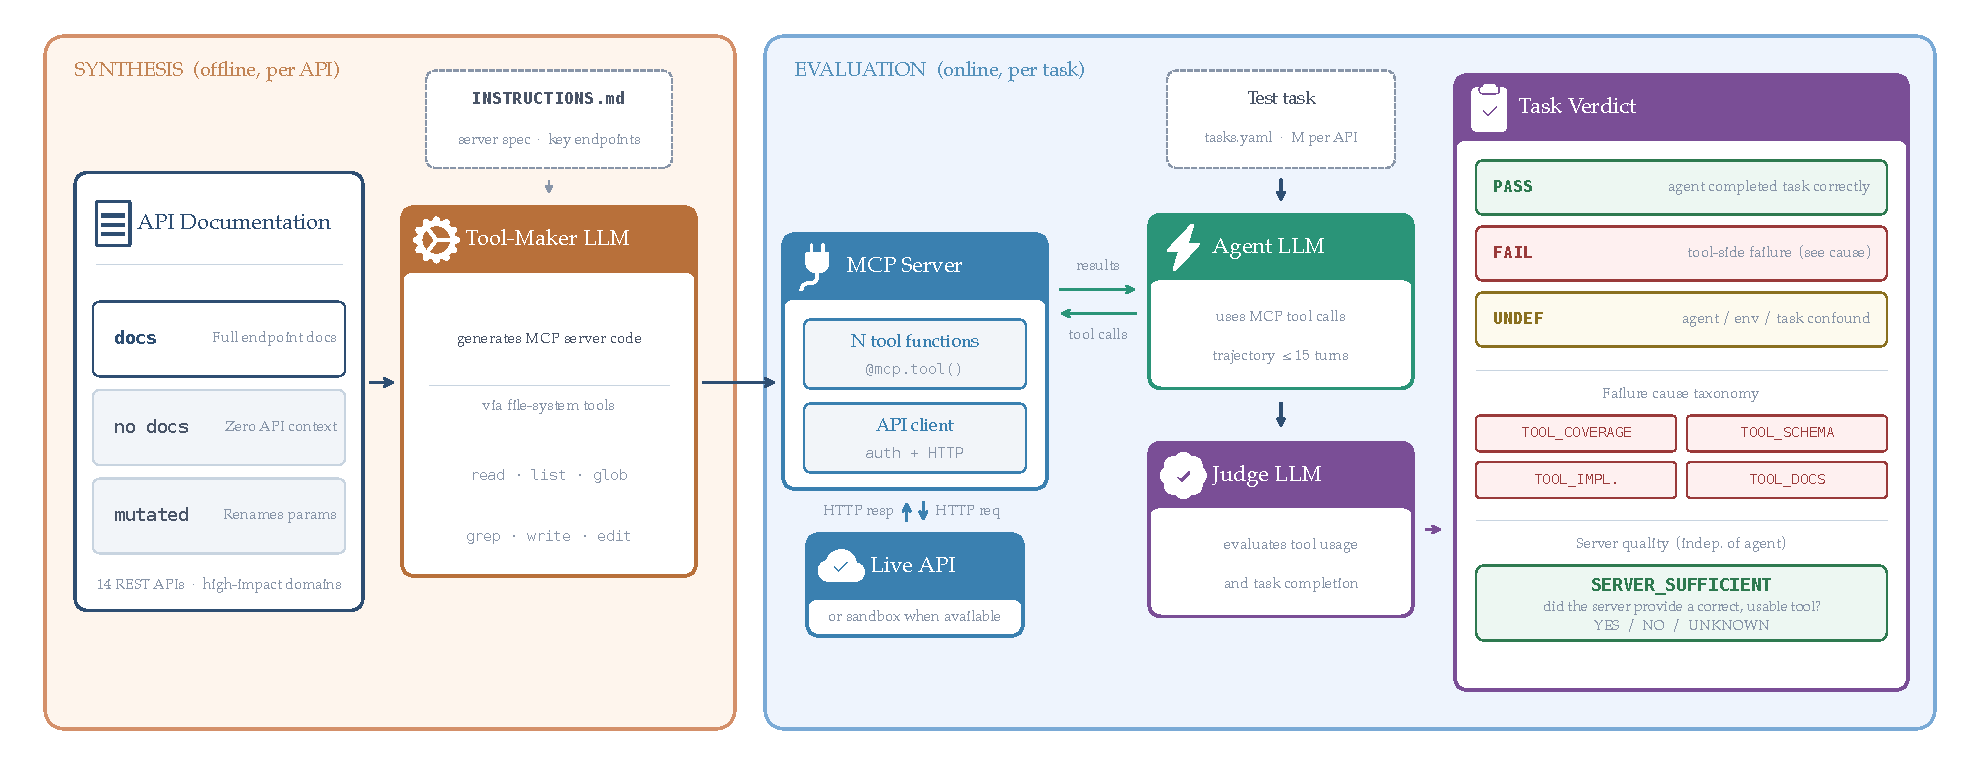
\includegraphics[width=\linewidth]{media/benchmark_pipeline_thesis_v4.pdf}
\caption{End-to-end benchmark pipeline. A synthesis agent reads documentation and produces an MCP server; a separate evaluation agent attempts tasks against it; a judge scores each attempt.}
\label{fig:pipeline}
\end{figure}

\noindent
This separation is the central design choice. In prior tool-use evaluations, the tool layer is given; here it is produced under test. A synthesized server that crashes, exposes incomplete tool coverage, or maps arguments incorrectly will cause agent failures regardless of how capable the evaluation model is. By isolating the synthesis stage, we can attribute failures to either the tool infrastructure (synthesis failures) or the evaluation agent (reasoning failures), and measure how tightly the two are coupled.

\section{Benchmark Datasets}

\subsection{API Selection}

We select 14 REST APIs spanning five domains: developer tooling (GitHub), productivity and collaboration (Notion, Confluence, Jira), e-commerce (eBay Buy, eBay Commerce, eBay Sell, Shopify), communication (Mastodon, Zulip), and data and financial services (Stripe, Alphavantage, Spoonacular, OpenWeatherMap). Selection criteria were: (i)~availability of a sandboxed or resettable test environment with stable test credentials, (ii)~REST-based HTTP interface returning JSON, (iii)~public developer documentation available as HTML or Markdown, and (iv)~variation along the two primary experimental axes: \emph{familiarity} (the degree to which an API is likely well-represented in pre-training corpora) and \emph{complexity} (endpoint count, parameter density, and authentication complexity).

APIs range from high-familiarity, high-complexity (GitHub, Stripe) to low-familiarity, low-complexity (Alphavantage, OpenWeatherMap). The eBay suite provides three difficulty tiers within a single platform: the Buy, Commerce, and Sell sub-APIs differ substantially in documentation volume and endpoint coverage despite sharing the same host and OAuth model. Jira and the eBay Sell API represent the most challenging synthesis targets, with large hierarchical documentation and high parameter cardinality.

\subsection{Documentation Collection}

For each API, we scrape the official developer documentation portal and convert it to Markdown using a DOM-to-Markdown pipeline. Depending on the API's documentation structure, this produces between 7 and 190 Markdown files per dataset (median approximately 35 files). Files range from single-endpoint reference pages to category-level overview pages covering multiple related endpoints. We do not post-process or selectively filter the scraped content beyond format normalisation; the synthesizer receives the documentation in the same form it appears online, including navigation artefacts, code samples in multiple languages, and pagination boilerplate.

This choice is deliberate: it reflects realistic synthesis conditions, where a practitioner points a synthesis agent at a raw documentation URL rather than a curated, cleaned API description. The resulting noise is part of the synthesis challenge the model must handle.

\subsection{Human Reference Servers}

For two APIs --- GitHub and Zulip --- publicly available, community-maintained MCP servers exist and can be evaluated against the same task suite. The GitHub MCP server is the official implementation maintained by GitHub; the Zulip server is a community-contributed open-source project. Both are written in TypeScript using the official MCP SDK and expose a subset of the respective APIs as tools. We run both reference servers against the same evaluation agent and judge pipeline used for the synthesized servers, without any modification.

These human-authored servers serve as a practical baseline: they represent what a developer with API familiarity and access to the official documentation would produce without time pressure from an automated benchmark. Crucially, neither server was constructed with our specific evaluation tasks in mind, so coverage gaps reflect genuine tool-design choices rather than benchmark overfitting. Comparing synthesized server PASS rates against these baselines directly answers whether automated synthesis can match or exceed hand-crafted implementations (Section~\ref{sec:rq2}).

\subsection{Parameter Mutations}

To probe the degree to which synthesis models rely on parametric knowledge rather than the provided documentation, we introduce a \emph{mutated} condition ($C_{\text{mut}}$) for each API. For each dataset, we identify 4--6 core parameter names that are prominent in the API and likely encoded in training-time weights (e.g.\ \texttt{limit}, \texttt{offset}, \texttt{sort} for eBay Buy) and replace them uniformly throughout the documentation with plausible but distinct alternatives (e.g.\ \texttt{max\_results}, \texttt{skip}, \texttt{order\_by}). Replacement names are chosen to be syntactically plausible --- consistent with conventions in adjacent APIs --- while being clearly different from the originals at the string level.

A synthesis model that faithfully follows the mutated documentation should produce tools using the new parameter names consistently. A model dominated by parametric memory will reproduce the original names regardless. We quantify this as \emph{mutation adherence}, measured at two levels:

\begin{itemize}
  \item \textbf{Interface adherence}: the mutated name appears as a Python
    identifier in the MCP tool function signature, i.e.\ the evaluation agent
    sees and receives the renamed parameter.
  \item \textbf{HTTP adherence}: the mutated name appears as a quoted string
    key in the outbound HTTP request. This is a stricter criterion; a model
    may adopt the renamed identifier locally but revert to the original name
    when constructing the HTTP payload.
\end{itemize}

\noindent
HTTP adherence is always $\leq$ interface adherence. The gap between the two is informative: a large gap indicates the model partially follows documentation (adopting Python argument names) but reverts to training priors when constructing HTTP calls.

To enable fair PASS comparison across conditions, we apply a \emph{patch} step to mutated servers before evaluation: the original parameter names are restored in the source files, so the evaluation agent always calls the real API with the correct parameters regardless of whether the synthesizer adopted the mutations. Adherence is measured before patching; PASS is measured after.

\section{Synthesis Pipeline}

\subsection{Task Specification}

Each dataset includes a \texttt{TASK.md} file that provides the synthesis agent with all information needed to produce a functional server. The
specification covers: the target implementation framework (FastMCP for Python,
or the official \texttt{@modelcontextprotocol/sdk} for TypeScript), the list of available documentation files and their location, required environment variables (API keys, OAuth credentials, sandbox flags), authentication flow (typically OAuth~2.0 client credentials or a static API key), coverage expectations (broad CRUD on core resource types, support for multi-step workflows), and required deliverables.

Deliverables are uniform across all datasets and language choices:
\begin{itemize}
  \item \texttt{server.py} (or \texttt{server.ts}): the MCP entry point that
    registers all tools and starts the stdio server.
  \item \texttt{requirements.txt} (or \texttt{package.json}): pinned
    dependencies for reproducible installation.
  \item \texttt{grounding.json}: a manifest mapping every synthesized tool
    name to the source documentation file and HTTP endpoint it implements
    (e.g.\ \path{\{"doc": "docs/browse.md", "endpoint": "GET /buy/browse/v1/item\_summary/search"\}}).
\end{itemize}

\noindent
The grounding manifest enables two lightweight analyses. \emph{Citation validity} checks that each entry's \texttt{doc} field names a file that exists in the documentation corpus and that the \texttt{endpoint} field contains a syntactically plausible HTTP method--path string. \emph{Grounding coverage} checks that every synthesized tool has a corresponding entry --- i.e.\ the synthesizer claimed a source for each tool it produced. These checks do not verify that the implementation is faithful to the cited documentation, only that the synthesizer anchored each tool to \emph{some} real document and endpoint rather than producing an entry-free, free-form stub.

\subsection{Synthesis Agent}

The synthesis agent operates in an agentic loop with access to a set of file-system tools. The primary synthesis models (GPT-5.2, GPT-5.4, and Qwen3-Coder-Next via vLLM) are provided six tools: \texttt{read\_file}, \texttt{write\_file}, \texttt{edit\_file}, \texttt{glob}, \texttt{grep}, and \texttt{list\_directory}. The agent receives the task specification and, depending on the synthesis condition, a populated documentation directory. It iterates freely until it produces the required deliverables.

A typical synthesis run follows three phases. In the \emph{exploration} phase (turns 1--3), the agent reads \texttt{TASK.md}, lists the documentation directory, and reads a subset of files to understand the API's structure and authentication model. In the \emph{implementation} phase (turns 4--20), it writes tool modules and a shared HTTP client. In the \emph{finalisation} phase (last 2--3 turns), it assembles \texttt{server.py}, writes
\texttt{grounding.json} and \texttt{requirements.txt}, then performs a self-verification pass by rereading key files. Figure~\ref{fig:synth-trace} shows a representative trace.

\begin{figure}[h]
\centering
\small
\begin{verbatim}
[turn 1]  read_file(TASK.md)
[turn 1]  glob(docs/*.md)
[turn 2]  read_file(docs/browse.md)
[turn 2]  read_file(docs/item.md)
[turn 4]  write_file(generated_tools/browse.py)
[turn 7]  write_file(generated_tools/order.py)
[turn 9]  write_file(server.py)
[turn 10] write_file(grounding.json)
[turn 11] write_file(requirements.txt)
\end{verbatim}
\caption{Typical synthesis agent trace (eBay Buy, docs condition, GPT-5.2). 813K input tokens, 11K output tokens, 190 seconds.}
\label{fig:synth-trace}
\end{figure}

\noindent
GPT-class synthesizers tend to produce a two-layer architecture: a \texttt{generated\_tools/} directory of domain-specific Python modules (e.g.\ \texttt{issues.py}, \texttt{pulls.py} for GitHub), each implementing a group of related endpoints through a shared HTTP client, with \texttt{server.py} acting as a thin registration layer applying \texttt{@mcp.tool()} decorators. Qwen3-Coder-Next typically produces a flat structure with all tool logic in a single \texttt{server.py}. Both patterns are accepted by the evaluation harness; only the MCP interface contract matters for evaluation.

\subsection{Synthesis Conditions}

We evaluate each API under three synthesis conditions, corresponding to three
instantiations of the context $C$ in Equation~\ref{eq:synthesis}:

\begin{itemize}
  \item $C_{\text{docs}}$ \textbf{(with docs)}: the agent receives all
    scraped documentation files in addition to the task specification.
  \item $C_{\emptyset}$ \textbf{(no docs)}: the agent receives only the
    task specification, with no documentation. All tool implementations must
    come from parametric knowledge.
  \item $C_{\text{mut}}$ \textbf{(mutated docs)}: the agent receives the
    mutated documentation, creating a controlled conflict between in-context
    parameter names and training-time priors.
\end{itemize}

\noindent
Synthesis resource usage varies substantially across conditions. GPT-5.2 docs-condition runs typically require 15--25 agent turns, consuming 14K--2.4M input tokens (reflecting documentation corpus size, which ranges from 7 to 190 files). No-docs runs are substantially shorter: 14K--24K input tokens and approximately 1 minute wall time, since the agent skips document reads and writes directly from parametric memory.

\subsection{Synthesis Models}

We evaluate five synthesis models. GPT-5.2 serves as the primary baseline, run across all 14 APIs and all three conditions. GPT-5.4 is run across all 14 APIs as a more recent baseline. Sonnet~4.6 (Claude Sonnet) is run across a representative subset of APIs. Gemini~3.1~Pro provides a third model family for comparison. Qwen3-Coder-Next is run locally via a vLLM inference server. These span a range of training corpora, post-training regimes, and context window sizes, allowing us to assess whether synthesis quality is model-specific or reflects a more general capability. Model comparison results are presented
in Section~\ref{sec:rq1}.

\section{Evaluation Framework}

\subsection{Evaluation Tasks}

For the 14 APIs in the primary evaluation set, we manually authored 13--25
natural-language tasks per API (265 tasks total; median 19 per API). Tasks
are specified in a \texttt{tasks.yaml} file using a four-field schema:

\begin{verbatim}
- id: search_products
  prompt: >
    Search for "wireless headphones" on eBay. Report
    the title, price, and item ID of the first 5
    results.
  expected: itemId
  tags: [read]
\end{verbatim}

\noindent
Tasks follow four design principles. First, prompts are \emph{goal-oriented}: they describe the desired outcome without naming tools, parameter fields, or HTTP endpoints. Second, they provide only the domain knowledge the agent cannot infer from tool schemas (e.g.\ ``amounts are in cents''), not call sequences or parameter names. Third, they require \emph{synthesis over echo}: comparison, counting, filtering, or multi-step retrieval rather than raw
response reporting. Fourth, chain depth is capped at six sequentially dependent calls, with the intended range being 2--4 steps.

The \texttt{expected} field contains a task-specific substring --- typically a field name, ID, or derived value --- that can only appear in the agent's final answer if it called the correct tool with semantically correct parameters. This string is passed to the judge as a ground-truth hint, reducing ambiguity in open-ended response scoring.

Tasks are distributed across four functional categories: smoke tests (single-call reads verifying basic tool reachability), multi-step workflows (search then retrieve, create then verify), error-handling tasks (invalid IDs, missing resources, permission boundaries), and harder synthesis tasks requiring pagination, cross-resource joins, or derived computations. Write tasks use a consistent naming prefix (e.g.\ \texttt{"Agent Eval Test *"}) to facilitate cleanup and prevent cross-run contamination.

\subsection{Evaluation Agent}

The evaluation agent (Gemini~2.5~Pro) connects to the synthesized MCP server via stdio transport and executes an agentic loop. At each turn it receives the full message history --- system prompt, task prompt, and all prior tool results as \texttt{ToolMessage} objects --- and responds with either a set of tool calls or a final textual answer. The loop terminates when the model emits a response with no tool calls, or after a maximum of 15 turns.

The agent's system prompt instructs it to always call at least one tool before answering, use observed tool results to inform subsequent calls, and pass environment-specific constants (e.g.\ \texttt{EBAY\_ENVIRONMENT=SANDBOX}) verbatim rather than inferring them. The prompt does not describe individual tools or their signatures; the agent discovers available tools at runtime by calling \texttt{list\_tools()}. The agent does not perform explicit chain-of-thought reasoning steps between tool calls; reasoning is implicit in the model's generation.

The evaluation harness speaks only MCP: it calls \texttt{list\_tools()} to discover available tools and \texttt{call\_tool(name, args)} to invoke them.
No other protocol or API client is provided. All HTTP logic --- authentication, request construction, token refresh, error handling --- executes inside the synthesized server process and is invisible to both the harness and the evaluation agent. The evaluation agent's performance therefore depends entirely on the interface quality and implementation correctness of the synthesized server.

\subsection{Judge}

Task outcomes are assessed by a separate LLM judge (Gemini~3~Flash) that does not participate in the agentic loop. The judge receives a structured prompt containing four components: the original task prompt, the list of all tool names and their one-line descriptions (from \texttt{list\_tools()}), the full tool-call trajectory formatted as numbered steps (\texttt{Step N: tool\_name(\{args\}) $\rightarrow$ [truncated result]}), and the agent's final textual answer. It is asked three questions:

\begin{enumerate}
  \item \textbf{OUTCOME}: Did the agent complete the task correctly?
    (\textsc{pass} / \textsc{fail})
  \item \textbf{FAILURE\_CAUSE}: If \textsc{fail}, what was the primary cause?
    One of eight codes:
    \textsc{tool\_coverage} (required tool absent from server),
    \textsc{tool\_documentation} (tool present but name or description
    prevented the agent from identifying it),
    \textsc{tool\_schema} (tool present but parameters incorrectly typed
    or named),
    \textsc{tool\_implementation} (tool called correctly but returned wrong
    or malformed data),
    \textsc{agent\_reasoning} (tools were sufficient but agent misused them),
    \textsc{task\_ambiguous} (task wording unclear or contradictory),
    \textsc{environment} (server crash, network error, credential failure),
    \textsc{none} (used when \textsc{outcome} is \textsc{pass}).
  \item \textbf{SERVER\_SUFFICIENT}: Setting aside what the agent did,
    did the synthesized server provide all tools needed to complete the task?
    (\textsc{yes} / \textsc{no} / \textsc{unknown})
\end{enumerate}

\noindent
The judge responds in a fixed plain-text format (no markdown) to enable reliable parsing:

\begin{verbatim}
OUTCOME: PASS
FAILURE_CAUSE: NONE
SERVER_SUFFICIENT: YES
REASON: The agent correctly identified the search tool, 
        applied the right filters, and extracted the 
        requested itemId values.
\end{verbatim}

\noindent
The \textsc{tool\_documentation} category distinguishes a missing tool (coverage gap) from a present-but-undiscoverable tool (documentation gap): when the server implements the correct endpoint but gives it a misleading name or description, the agent fails not because the tool is absent but because it cannot identify it. This distinction is absent from most prior tool-use benchmarks and matters for understanding where synthesis quality breaks down independent of coverage.

\subsection{Metrics}
\label{sec:metrics}

We report two primary metrics derived from the judge's structured output.

\textbf{PASS} is the fraction of task attempts scored \textsc{pass} out of all \emph{scoreable} attempts. A task attempt is excluded from the denominator if it is attributed to \textsc{environment} (external infrastructure failure unrelated to synthesis quality) or \textsc{task\_ambiguous} (measurement
confound). Failures attributed to \textsc{agent\_reasoning} are also excluded:
they count neither as pass nor fail, because they reflect the evaluation agent's behaviour rather than the synthesized server. PASS is thus a clean signal about tool infrastructure quality:
%
\begin{equation}
  \text{PASS}
  = \frac{\#\,\textsc{pass}}
    {\#\,\textsc{pass} + \#\,\textsc{fail}_{\text{tool}}}
  \label{eq:pass}
\end{equation}
%
where $\#\,\textsc{fail}_{\text{tool}}$ counts failures attributed to
\textsc{tool\_coverage}, \textsc{tool\_documentation},
\textsc{tool\_schema}, or \textsc{tool\_implementation}.

\textbf{SYNTH} (synthesis sufficiency) is derived from the \textsc{server\_sufficient} verdict: it is the fraction of tasks for which the judge found the server sufficient regardless of whether the agent succeeded. SYNTH measures synthesis quality independently of the evaluation
agent, and is computed only for tasks where the judge returned a non-\textsc{unknown} verdict. When SYNTH is high but PASS is low, the bottleneck is agent reasoning; when both are low, the bottleneck is synthesis.

Together, the two metrics place each API--condition data point in one of three regimes: \emph{synthesis-limited} (low SYNTH, low PASS), \emph{agent-limited} (high SYNTH, lower PASS), or \emph{ceiling} (high SYNTH, high PASS). The scatter plot of SYNTH against PASS (Section~\ref{sec:rq5}) visualises this decomposition across all 42 API--condition pairs in the primary evaluation.

        \chapter{Results}
\label{sec:results}
% Give the outcomes for each research question in the form of a table or graphic (with caption).
%Write about your results here. Good captions to tables and/or figures are key.

% Sometimes,  especially  if  you  have  quite  different experiments or research  questions,  it makes sense to interleave the experimental setup and the results sections, so the reader does not get lost. It is then helpful to structure clearly in (sub)subsections.

%\section{Table and Figures}
%        \begin{table}[h] % h for Here, t for Top, b for Bottom
%                \centering
%                \caption{By convention, Table caption goes on top.}
%                \begin{tabular}{lcr}
%                        \textbf{Left} & \textbf{center} & \textbf{right} \\
%                        \hline
%                        111 & 222 & 333 \\
%                        444 & 555 & 666
%                \end{tabular}
%        \end{table}

%        \begin{figure}[h]
%                \centering
%                \includegraphics[width=0.5\linewidth]{example-image}
%                \caption[Example figure]{Example figure. Notice that the caption goes below and that there is a way to have a shorter caption for the list of Figures.}
%        \end{figure}

%        \begin{figure*}[b]
%                \centering
%                \includegraphics[width=0.8\linewidth, height=.2\textheight]{example-image}
%                \caption{Example figure spanning the two columns.}
%        \end{figure*}


This chapter presents results for the five research questions introduced before. Section~\ref{sec:rq1} establishes that synthesis is feasible for most APIs. Section~\ref{sec:rq2} shows that synthesized
servers enable effective agent task completion and compares against
human-authored references. Section~\ref{sec:rq3} characterises how
synthesizers rely on parametric knowledge and when this affects downstream
performance. Section~\ref{sec:rq4} examines the effect of documentation
availability. Section~\ref{sec:rq5} quantifies the relationship between
synthesis quality and agent pass rate.
Section~\ref{sec:model_comparison} extends the analysis to seven synthesis models
on a common three-API evaluation set.

% ------------------------------------------------------------
\section{RQ1: Synthesis Feasibility}
\label{sec:rq1}
% ------------------------------------------------------------

\textbf{Can LLMs synthesize functional API tool servers from documentation alone?}

Figure~\ref{fig:heatmap} shows PASS and SYNTH across all 14 APIs and three
synthesis conditions. Twelve of 14 APIs achieve SYNTH $\geq 75\%$ in the
docs condition, with a median of approximately 84\%. Only Jira (56\%) and
eBay Sell (43\%) fall consistently below that threshold, indicating that
synthesis is feasible for the large majority of APIs tested.

The dominant failure mode is \emph{coverage gap}: the server starts and
runs correctly, but the synthesizer omits the specific endpoints required
by certain benchmark tasks. This is most pronounced for large APIs with many endpoints (eBay Sell, Jira), consistent with the negative trend between
endpoint count and SYNTH visible in Figure~\ref{fig:complexity}. Structural
failure --- servers that crash or omit the required \texttt{server.py}
entrypoint entirely --- is rare with GPT-5.2 (the primary synthesis model)
and occurs mainly with weaker or smaller models.

SYNTH is also notably stable across conditions for most APIs: Confluence
holds at 95\% across all three conditions and Mastodon at 93--100\%,
indicating that synthesis quality is primarily determined by API structure
rather than what context is provided. The exceptions --- eBay Commerce drops from SYNTH=100\% (docs) to 54\% (mutated) --- arise where parameter
mutations reduce tool coverage directly.

Grounding analysis shows that synthesizers consistently anchor tools to
real documentation sources: citation validity is 86--100\% across datasets
(every \texttt{grounding.json} entry points to an existing file with a
syntactically plausible endpoint string), and grounding coverage is complete (every synthesized tool has a corresponding entry). This rules out the possibility that high SYNTH scores are driven entirely by tools whose implementations are unmoored from any documentation --- though it does not verify that each tool correctly implements what its cited document describes. Even in the no-docs condition, SYNTH remains high for well-known APIs (GitHub nodocs SYNTH=87\%), suggesting that parametric knowledge can partially substitute for documentation at the synthesis stage --- a finding developed further in Section~\ref{sec:rq3}.

\begin{table}[htbp]
  \centering
  \caption{Agent pass rate (PASS, \%) per API and synthesis condition.
    Rows sorted by mean PASS descending. \textbf{Bold} marks the highest
    value in each row. \colorbox{red!12}{Red} cells indicate PASS $< 50\%$.
    PASS = agent pass rate on scoreable tasks. Heatmap (Fig.~\ref{fig:heatmap}) shows SYNTH alongside PASS.}
  \label{tab:pass_results}
  \setlength{\tabcolsep}{5pt}
  \small
  \begin{tabular}{lrrr}
    \toprule
    \textbf{Dataset} & \textbf{With docs} & \textbf{No docs} & \textbf{Mutated params} \\
    \midrule
    Mastodon         & \textbf{100} & \textbf{100} & \textbf{100} \\
    OpenWeatherMap   & \textbf{100} &           86 & \textbf{100} \\
    Spoonacular      & \textbf{100} &           90 &           78 \\
    Notion           &           78 & \textbf{100} & \textbf{100} \\
    Confluence       &           92 &           93 & \textbf{91}  \\
    Alphavantage     &           86 &           90 & \textbf{88}  \\
    eBay Commerce    & \textbf{100} &           89 &           55 \\
    Shopify          &           87 & \textbf{92}  &           62 \\
    GitHub           &           62 & \textbf{83}  &           76 \\
    eBay Buy         &           73 &           67 & \textbf{80}  \\
    Zulip            & \textbf{80}  &           60 &           62 \\
    Stripe           & \textbf{72}  &           62 &           57 \\
    eBay Sell        &           38 & \textbf{50}  & \cellcolor{red!12}43 \\
    Jira             & \textbf{50}  & \cellcolor{red!12}25 & \textbf{50} \\
    \midrule
    \textit{Median}  &           80 &           86 &           77 \\
    \bottomrule
  \end{tabular}
\end{table}

\begin{figure}[htbp]
  \centering
  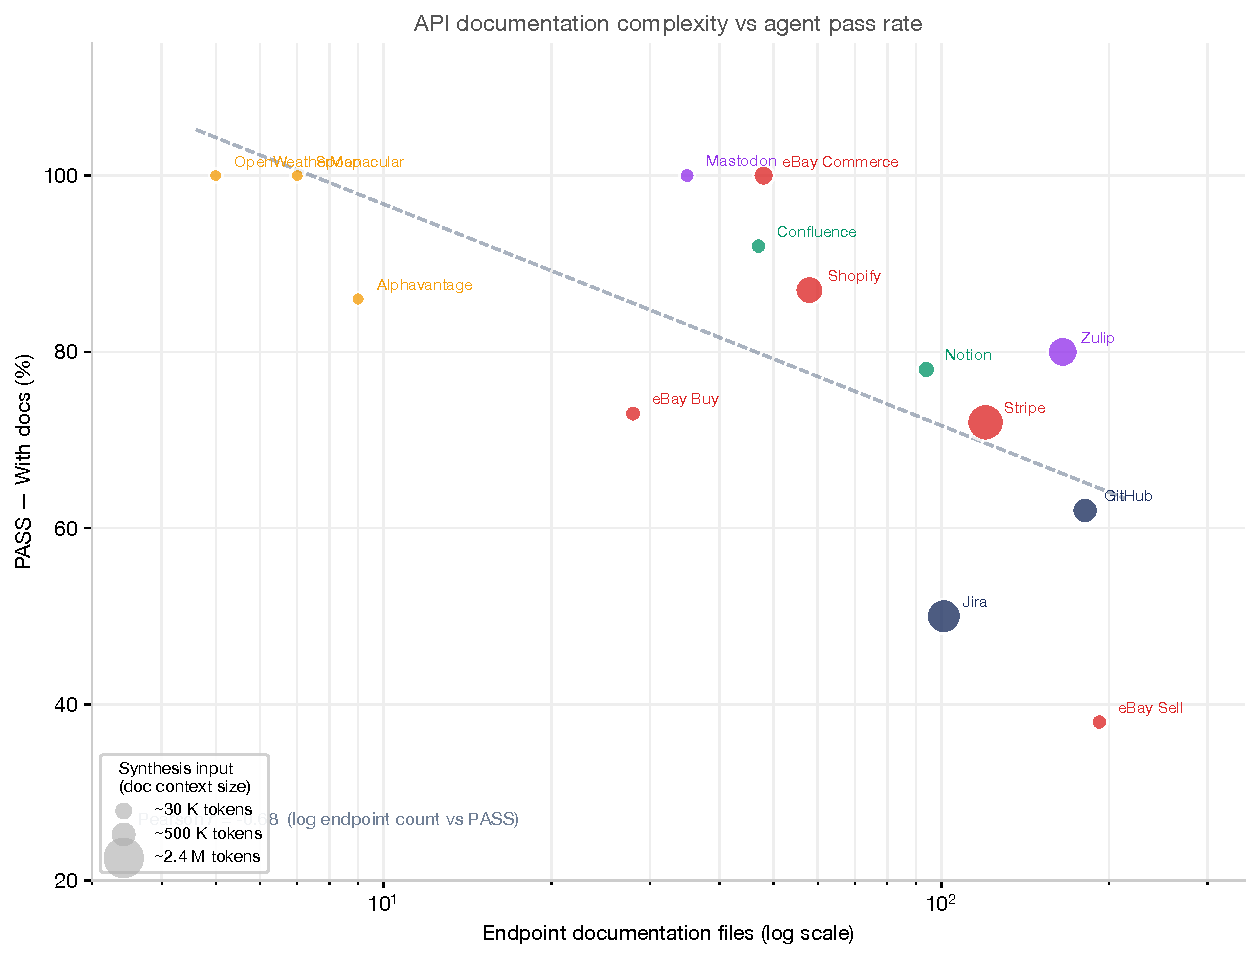
\includegraphics[width=\linewidth]{media/fig8_api_complexity.pdf}
  \caption{Endpoint documentation file count (log scale) vs.\ agent pass rate
    (docs condition). Marker size encodes synthesis input token volume.
    Dashed line is a log-linear fit. Larger APIs with denser documentation
    systematically yield lower PASS, driven by coverage gaps rather than
    server errors.}
  \label{fig:complexity}
\end{figure}

\begin{figure}[htbp]
  \centering
  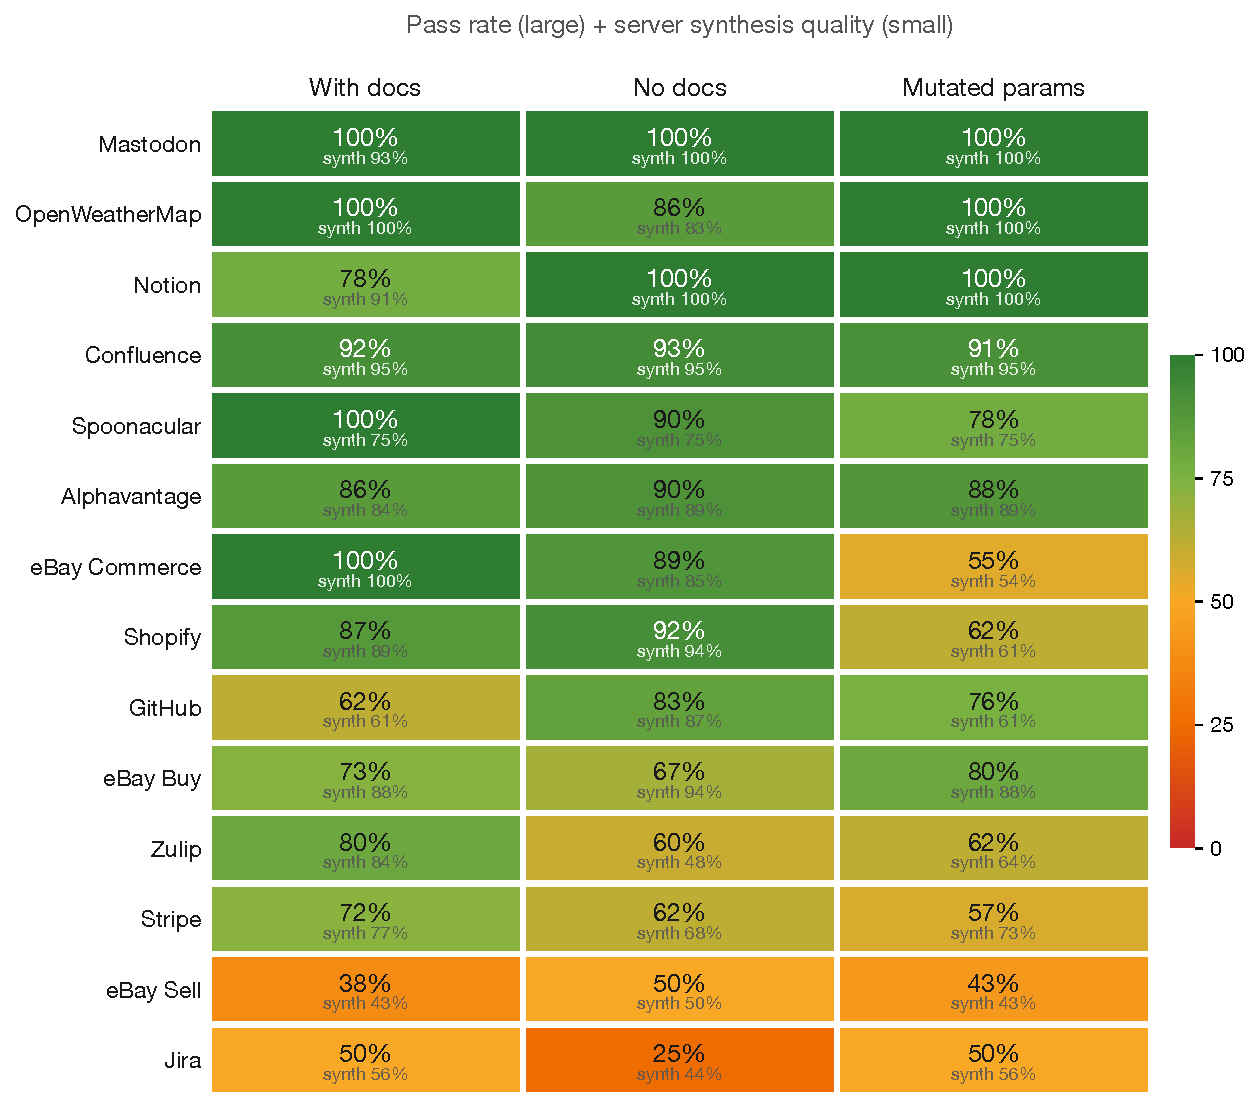
\includegraphics[width=\linewidth]{media/fig1_primary_heatmap.pdf}
  \caption{Agent pass rate (PASS, large) and server synthesis sufficiency
    (SYNTH, small) across 14 APIs and three synthesis conditions.
    Rows sorted by mean PASS descending.
    Colour encodes PASS on a red--orange--green scale.}
  \label{fig:heatmap}
\end{figure}

% ------------------------------------------------------------
\section{RQ2: Agent Task Completion}
\label{sec:rq2}
% ------------------------------------------------------------

\textbf{Do synthesized servers enable effective agent task completion, compared to human-authored references?}

Figure~\ref{fig:strip} shows the distribution of PASS across APIs and conditions. The median PASS is approximately 80\% in the docs condition and 86\% in the no-docs condition, with a long tail of high performers (Mastodon 100\% across all three conditions; Confluence 91--93\%; OpenWeatherMap 86--100\%) and a small floor group (Jira mean 42\%; eBay Sell mean 45\%).

The variance across APIs is explained by two distinct mechanisms. For the floor group, SYNTH is also low: Jira SYNTH=44--56\%, eBay Sell SYNTH=43\%. These are synthesis failures masquerading as agent failures --- when the required tools are absent, the agent cannot compensate. For APIs with moderate PASS but higher SYNTH (Stripe: SYNTH=77\%, PASS=72\%), the bottleneck shifts to agent reasoning on complex multi-step tasks. Figure~\ref{fig:scatter} makes this distinction visible: points near the diagonal are synthesis-limited; points below it are agent-limited.

\begin{figure}[htbp]
  \centering
  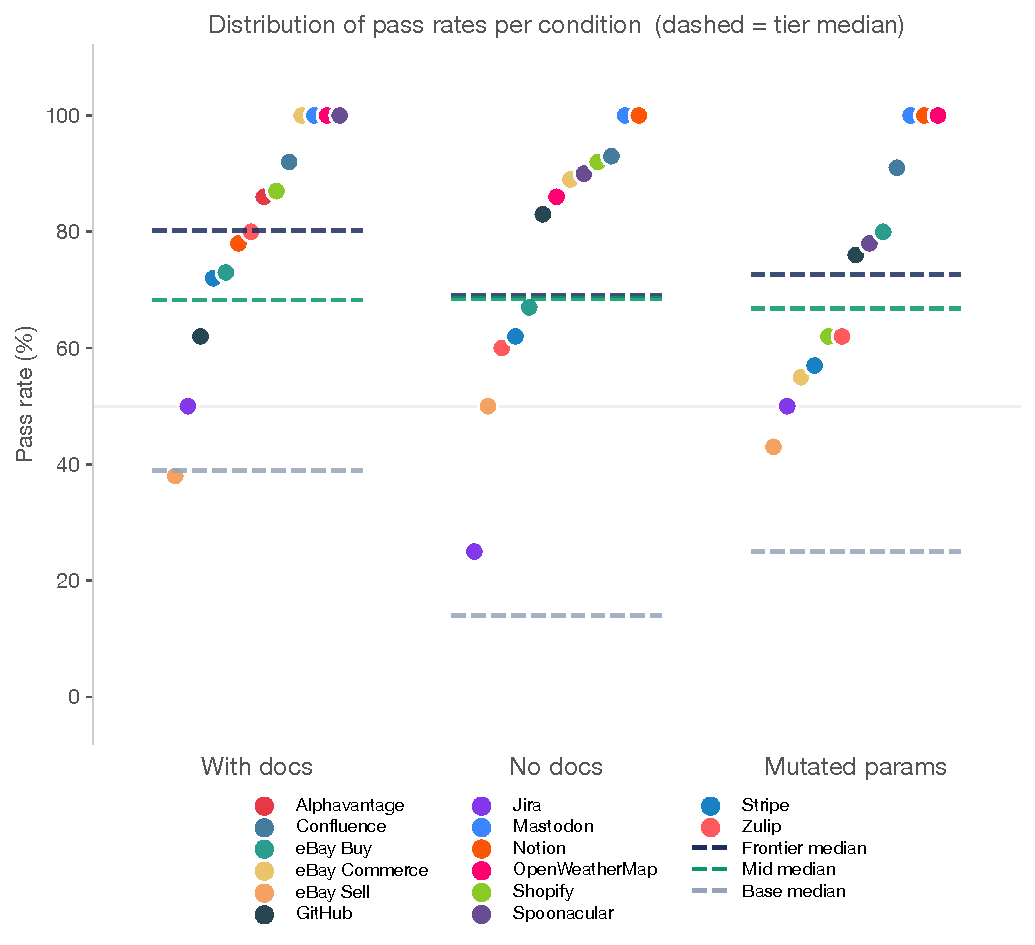
\includegraphics[width=0.85\linewidth]{media/fig2_condition_slopes.pdf}
  \caption{Distribution of PASS per synthesis condition.
    Each dot is one API; dashed line shows the median.
    The 50\% reference line is shown in light grey.}
  \label{fig:strip}
\end{figure}

\paragraph{Comparison with human-authored references.}
On GitHub, the community MCP server scores 65\% PASS. Synthesized servers with docs match this (62--67\% across valid runs), and synthesized servers without docs comfortably exceed it (83--90\%), because the synthesis model's parametric knowledge of the GitHub API produces more complete tool coverage than the hand-written reference. On Zulip, the community reference scores 68\%; the synthesized docs-condition server scores 80\%. In both cases the human reference fails on the same \texttt{TOOL\_COVERAGE} pattern --- missing webhooks, branch protection, and Actions dispatch for GitHub; message edit, DM search, and scheduled messages for Zulip ---while the synthesized server adds these endpoints.

% ------------------------------------------------------------
\section{RQ3: Parametric Knowledge and Documentation Faithfulness}
\label{sec:rq3}
% ------------------------------------------------------------

\textbf{To what extent do synthesizers rely on parametric knowledge rather than documentation, and does this affect performance?}

The mutated-docs condition directly operationalises this question: if a synthesizer adopts the renamed parameter names, it is reading the documentation; if it does not, it is writing from memory. Figure~\ref{fig:adherence} shows the PASS delta (mutated $-$ docs) per API alongside the interface-layer adherence rate (diamond markers). GitHub, Stripe, Shopify, Zulip, and Jira show near-zero adherence --- the synthesizer ignores mutations entirely and writes from training-time knowledge. Mastodon and Alphavantage reach full adherence, indicating the model follows provided documentation faithfully for less-familiar APIs.

The bar lengths directly test whether low adherence implies immunity to mutation. GitHub fits: near-zero adherence, bar near zero ($-$14 pp, offset by nodocs improvements visible in Fig.~\ref{fig:docs_effect}). Stripe does not: also near-zero adherence, yet mutation still costs 15 pp. This confirms that parametric reliance at synthesis does not cleanly propagate to agent performance.

The mechanism behind this is that the effect of parametric reliance depends on whether the synthesis model and the evaluation agent share the same prior. When both ignore mutations and operate from training-time knowledge --- as for GitHub --- the mutation is invisible to the whole pipeline and performance is unaffected. When the synthesizer adopts mutations faithfully (high adherence) but the evaluation agent's prior does not anticipate the renamed parameters, performance degrades. The contamination is only detectable as a problem when the two components have mismatched priors.

\begin{figure}[htbp]
  \centering
  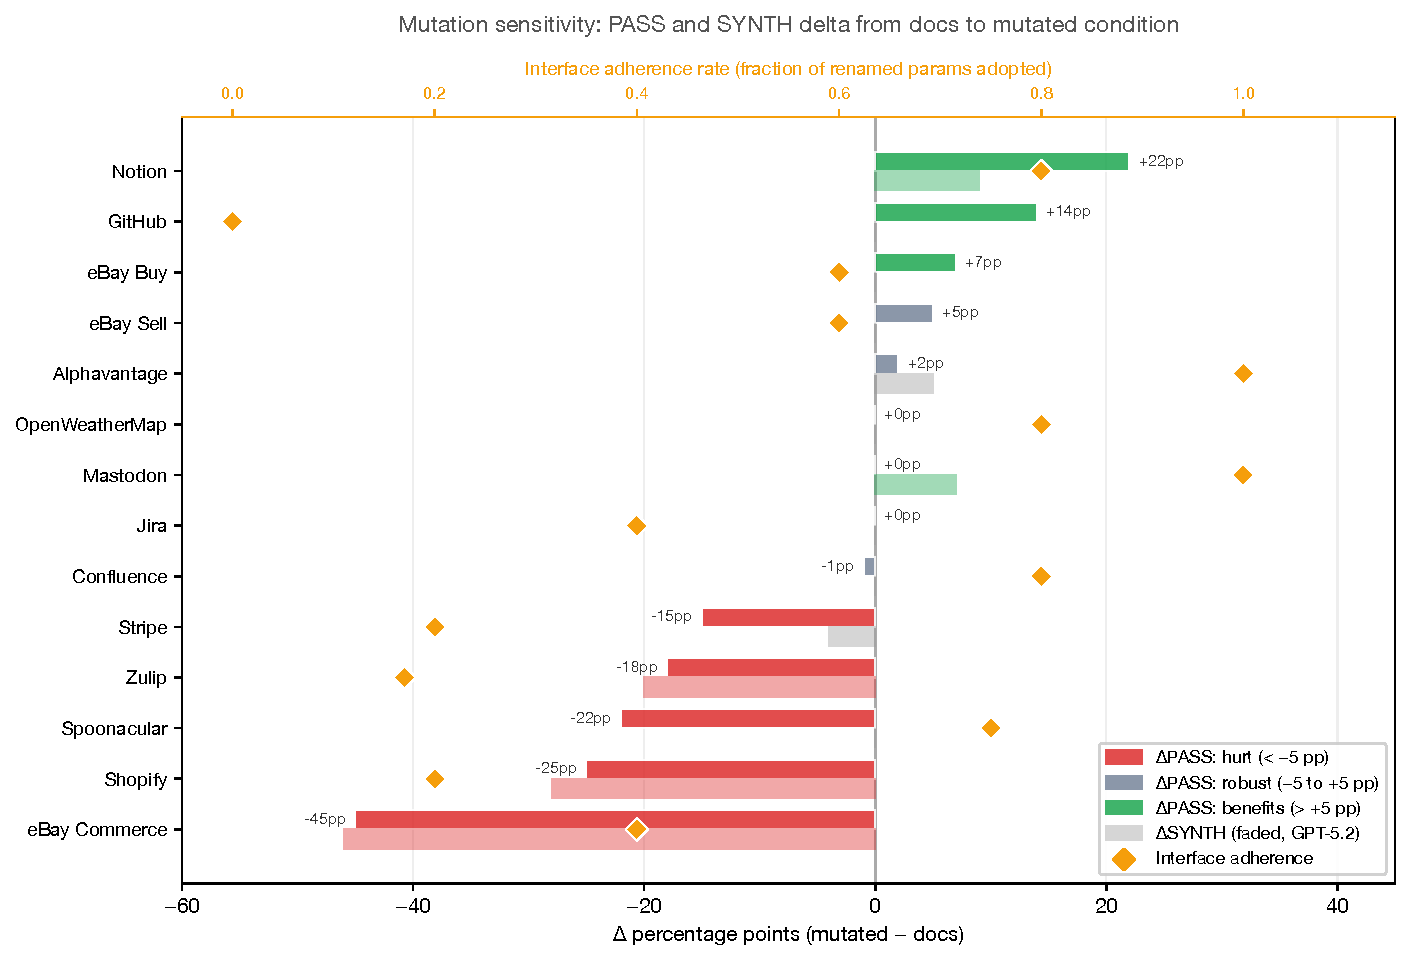
\includegraphics[width=\linewidth]{media/fig6_mutation_sensitivity.pdf}
  \caption{PASS delta (mutated $-$ docs, in percentage points) per API, sorted
    ascending. Red bars indicate APIs hurt by parameter renaming; green bars
    indicate APIs that benefit or are unaffected. Diamond markers (amber) show
    the interface-layer mutation adherence rate: how many renamed parameters the
    synthesizer adopted. Low adherence implies the synthesizer relied on
    parametric knowledge rather than the provided documentation.}
  \label{fig:adherence}
\end{figure}

% ------------------------------------------------------------
\section{RQ4: Effect of Documentation Availability}
\label{sec:rq4}
% ------------------------------------------------------------

\textbf{How does documentation availability affect synthesis and agent
performance?}

Figure~\ref{fig:strip} shows the median PASS per condition. The no-docs median (86\%) meets or exceeds the docs median (80\%), indicating that removing documentation does not on average degrade agent performance. This aggregate result conceals meaningful per-API variation, visible in Figure~\ref{fig:docs_effect}.

\begin{figure}[htbp]
  \centering
  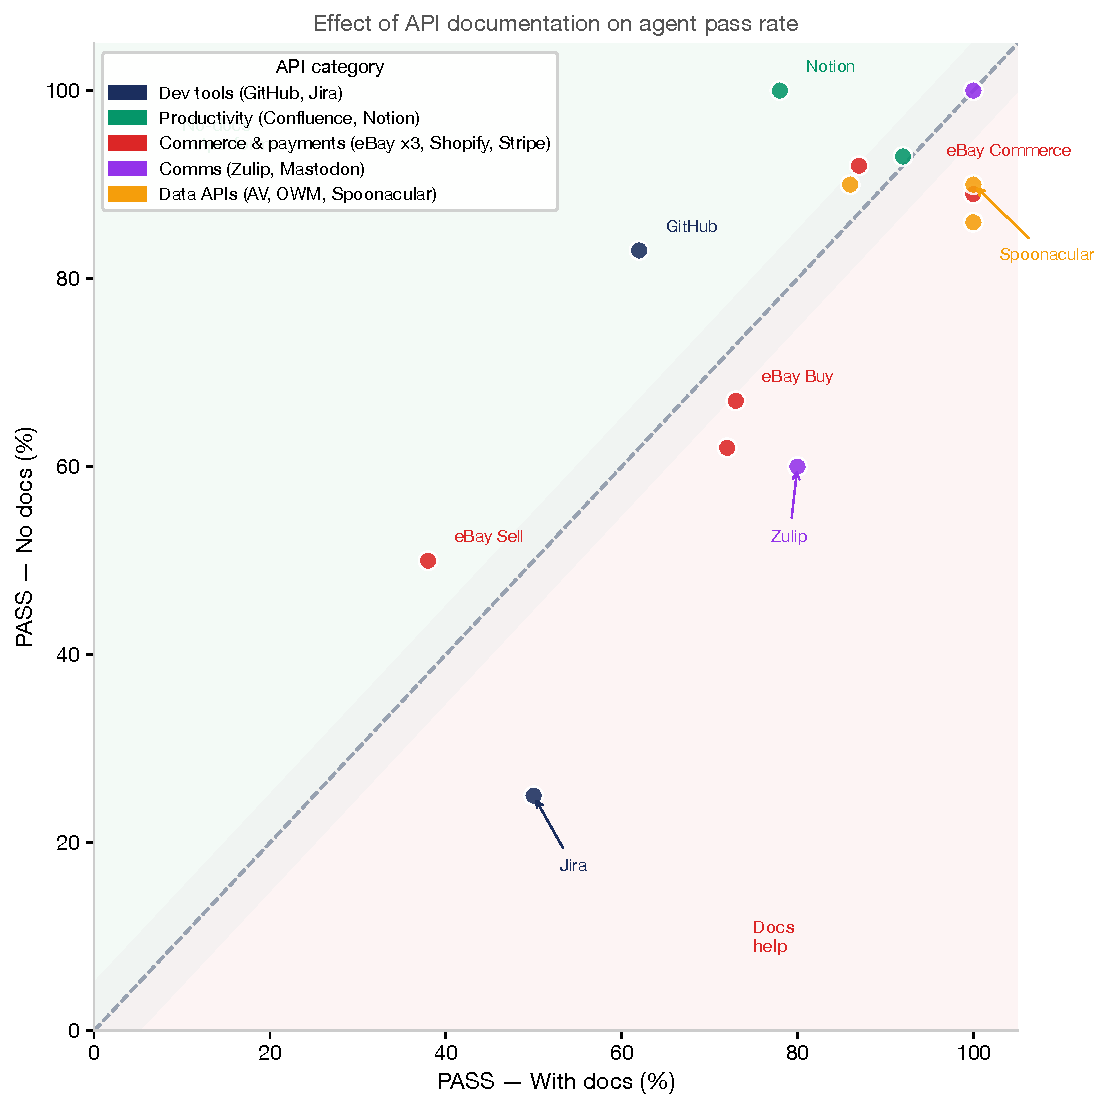
\includegraphics[width=0.72\linewidth]{media/fig7_docs_effect.pdf}
  \caption{Docs vs.\ no-docs PASS per API. Points above the diagonal
    indicate APIs where removing documentation improved performance;
    points below indicate APIs where documentation helped.}
  \label{fig:docs_effect}
\end{figure}

APIs above the diagonal (nodocs wins) include GitHub, Notion, and Mastodon: high-frequency, well-documented APIs for which the synthesis model has strong training-time priors. Removing documentation reduces noise and allows the model to produce a clean, complete server from memory. APIs below the diagonal (docs help) include Stripe and Zulip: less saturated in training
data, or with API conventions sufficiently idiosyncratic that documentation provides genuine signal the model could not otherwise recover.

The mutated condition (also visible in Figure~\ref{fig:strip}) shows a modest further decrease in the median (77\%), indicating that parameter renaming does introduce some degradation on average. However, the APIs most sensitive to mutation are precisely those with high adherence (Section~\ref{sec:rq3}), consistent with the interpretation that harm from mutations is mediated by whether the synthesizer adopted them.

% ------------------------------------------------------------
\section{RQ5: Synthesis Quality as a Predictor of Agent Performance}
\label{sec:rq5}
% ------------------------------------------------------------

\textbf{Does synthesis quality predict agent task performance?}

Figure~\ref{fig:scatter} plots SYNTH against PASS for all 42 API--condition pairs. The Pearson correlation is $r = 0.895$ ($p < 0.0001$, $n = 42$), indicating a strong linear relationship between synthesis sufficiency and agent pass rate. This is the central methodological validation result: SYNTH is a reliable proxy for downstream utility, and failures in synthesis propagate to agent failures with high fidelity.

\begin{figure}[htbp]
  \centering
  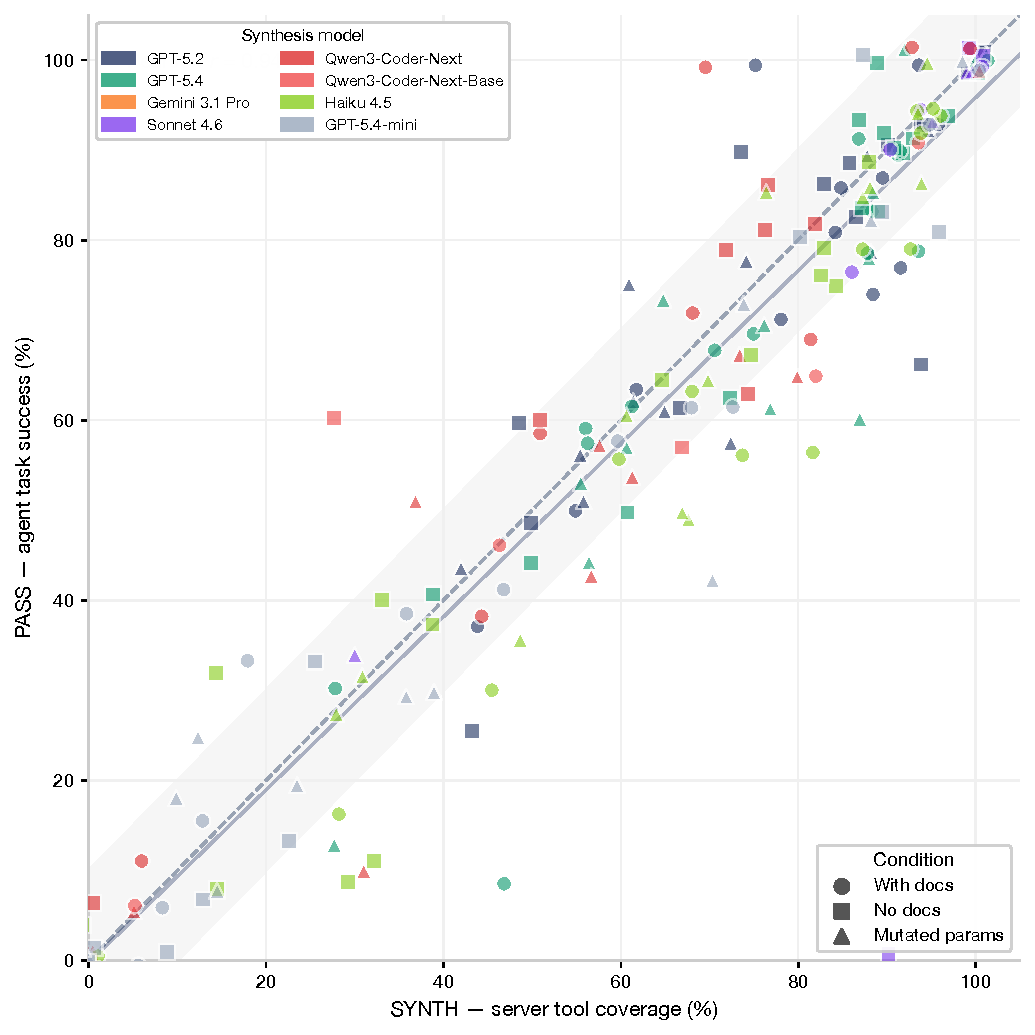
\includegraphics[width=0.72\linewidth]{media/fig4_synth_scatter.pdf}
  \caption{SYNTH vs.\ PASS across all 42 API--condition pairs
    ($r = 0.895$). Shape encodes synthesis condition;
    colour encodes API category.
    The dashed line is $y = x$; the grey band is $\pm 10$ pp.}
  \label{fig:scatter}
\end{figure}

The points near or above the diagonal represent cases where the agent performs at or above what synthesis quality would predict --- most commonly when the agent compensates for minor coverage gaps with general reasoning (Spoonacular: SYNTH=75\%, PASS=100\% in the docs condition). Points well below the diagonal (eBay Commerce mutated: SYNTH=54\%, PASS=55\%) confirm that when synthesis fails to cover the task space, agent performance cannot recover. The Jira no-docs outlier (SYNTH=44\%, PASS=25\%) represents the most severe case of synthesis-induced failure in the benchmark.

Taken together, these results validate SYNTH as a leading indicator: measuring synthesis sufficiency before running the full evaluation pipeline gives a reliable estimate of whether agent task completion will succeed.

% ------------------------------------------------------------
\section{Model Comparison}
\label{sec:model_comparison}
% ------------------------------------------------------------

\textbf{How does synthesis model capability affect agent pass rate?}

To isolate model effects from API-specific variation, we evaluate eight synthesis models on a common three-API set (GitHub, Stripe, Zulip) selected to span low, medium, and high familiarity. Table~\ref{tab:model_comparison} reports PASS for all models across all three APIs and conditions; absent conditions are synthesis failures (no runnable server produced) and score as 0\%. Figure~\ref{fig:model_capability} summarises the per-model distributions. Qwen3-Coder-Next-Base has very sparse coverage on this set --- GitHub produced no valid server in any condition, and only single conditions were evaluated for Stripe and Zulip --- reflecting the limits of a base model without instruction tuning.

Sonnet~4.6 achieves the highest median PASS across the three APIs. GPT-5.2, GPT-5.4, and Haiku~4.5 form a competitive mid-tier, though with distinct failure modes: GPT-5.4 produces broken tool stubs for Stripe docs (8\%) --- a synthesis-level failure confirmed by SYNTH=48\% --- while Haiku~4.5 collapses on Zulip nodocs (36\%) and mutated (26\%), indicating weaker parametric coverage of that API. Gemini~3.1 Pro is broadly competitive at mid-tier for GitHub and Zulip but weaker on Stripe.

The two weakest models show qualitatively different failure patterns. GPT-5.4-mini consistently produces shallow servers with too few relevant tools (TOOL\_COVERAGE dominates across all nine conditions, −43\,pp below GPT-5.2 on average). Qwen3-Coder-Next has high crash rates --- Stripe docs and mutated, and Zulip docs and nodocs all produce servers that fail on startup --- but achieves competitive results on the conditions where synthesis succeeds (GitHub: 57--60\%, Zulip mutated: 64\%, Stripe nodocs: 62\%).

Synthesis reliability --- the fraction of conditions producing a runnable server --- scales with model tier. Sonnet~4.6, GPT-5.2, and Gemini~3.1 Pro achieve near-complete reliability across all nine conditions. Qwen3-Coder-Next fails on four of nine; GPT-5.4-mini produces a server for all nine but with coverage too thin to be useful (SYNTH 14--48\%).

The nodocs advantage observed in RQ4 is strongest for larger models. Sonnet~4.6 and GPT-5.2 improve or hold steady on GitHub when documentation is removed, consistent with strong parametric priors overriding documentation noise. Qwen3-Coder-Next, by contrast, shows 60\% interface-layer adherence on GitHub and Stripe (though 0\% HTTP adherence --- the renamed parameters are reflected in Python signatures but not in outbound API calls), indicating it reads documentation more literally but does not fully propagate renames to execution.

This model-level variation in adherence is a confound when interpreting the aggregate adherence results in Section~\ref{sec:rq3}: the near-zero aggregate adherence for GitHub reflects a mixture of high-capability models ignoring mutations entirely (parametric dominance) and lower-capability models adopting renames at the interface level but not the HTTP level. The full per-model adherence breakdown is reported in Appendix~\ref{sec:apx:full_results}.

\begin{table}[htbp]
  \centering
  \caption{PASS (\%) on the common three-API set by synthesis model and condition.
    Models ordered by approximate capability (ascending left to right).
    0\% cells marked \colorbox{red!12}{red} include both true zeros and synthesis crashes.
    Shaded rows are the two weakest models.}
  \label{tab:model_comparison}
  \setlength{\tabcolsep}{3.5pt}
  \scriptsize
  \begin{tabular}{ll rrr rrr rrr}
    \toprule
    & & \multicolumn{3}{c}{\textbf{GitHub}} & \multicolumn{3}{c}{\textbf{Stripe}} & \multicolumn{3}{c}{\textbf{Zulip}} \\
    \cmidrule(lr){3-5}\cmidrule(lr){6-8}\cmidrule(lr){9-11}
    \textbf{Model} & & D & N & M & D & N & M & D & N & M \\
    \midrule
    \rowcolor{gray!10}
    GPT-5.4-mini          & & 38 & 32 & 30 & 14 & \cellcolor{red!12}0 & 19 & 40 & 14 & 29 \\
    \rowcolor{gray!10}
    Qwen3-Coder-Next-Base & & \cellcolor{red!12}0 & \cellcolor{red!12}0 & \cellcolor{red!12}0 & \cellcolor{red!12}0 & 56 & \cellcolor{red!12}0 & \cellcolor{red!12}0 & \cellcolor{red!12}0 & \cellcolor{red!12}0 \\
    \rowcolor{gray!10}
    Qwen3-Coder-Next      & & 58 & 60 & 57 & \cellcolor{red!12}0 & 62 & \cellcolor{red!12}0 & \cellcolor{red!12}0 & \cellcolor{red!12}0 & 64 \\
    Gemini~3.1 Pro        & & \textbf{78} & 71 & 36 & 47 & 50 & 59 & 76 & \textbf{84} & 62 \\
    GPT-5.2               & & 62 & 83 & 76 & \textbf{72} & 62 & 57 & \textbf{80} & 60 & 62 \\
    GPT-5.4               & & 58 & \textbf{89} & 73 & 8 & 62 & 12 & \textbf{90} & 85 & 71 \\
    Haiku~4.5             & & \textbf{95} & 90 & \textbf{86} & 57 & \textbf{75} & \textbf{86} & 55 & 36 & 26 \\
    Sonnet~4.6            & & 90 & \textbf{100} & \textbf{100} & 77 & \textbf{100} & \textbf{100} & \textbf{100} & 43 & \cellcolor{red!12}0 \\
    \bottomrule
  \end{tabular}
  \par\smallskip
  \raggedright\scriptsize D = docs, N = nodocs, M = mutated.
  Bold = highest per column. Shaded rows = weakest models.
  Qwen3-Coder-Next-Base GitHub: no server.py produced; Stripe/Zulip: only one condition evaluated.
  Sonnet~4.6 Zulip mutated: synthesis stream error on all attempts.
\end{table}

\begin{figure}[htbp]
  \centering
  
\includegraphics[width=\linewidth]{media/fig9_model_capability.pdf}
  \caption{PASS distributions for seven synthesis models on the common
    three-API set (GitHub, Stripe, Zulip), ordered by approximate capability.
    Each box shows nine data points (3 APIs $\times$ 3 conditions);
    crash/failure conditions count as 0\%.}
  \label{fig:model_capability}
\end{figure}

\begin{figure*}[htbp]
  \centering
  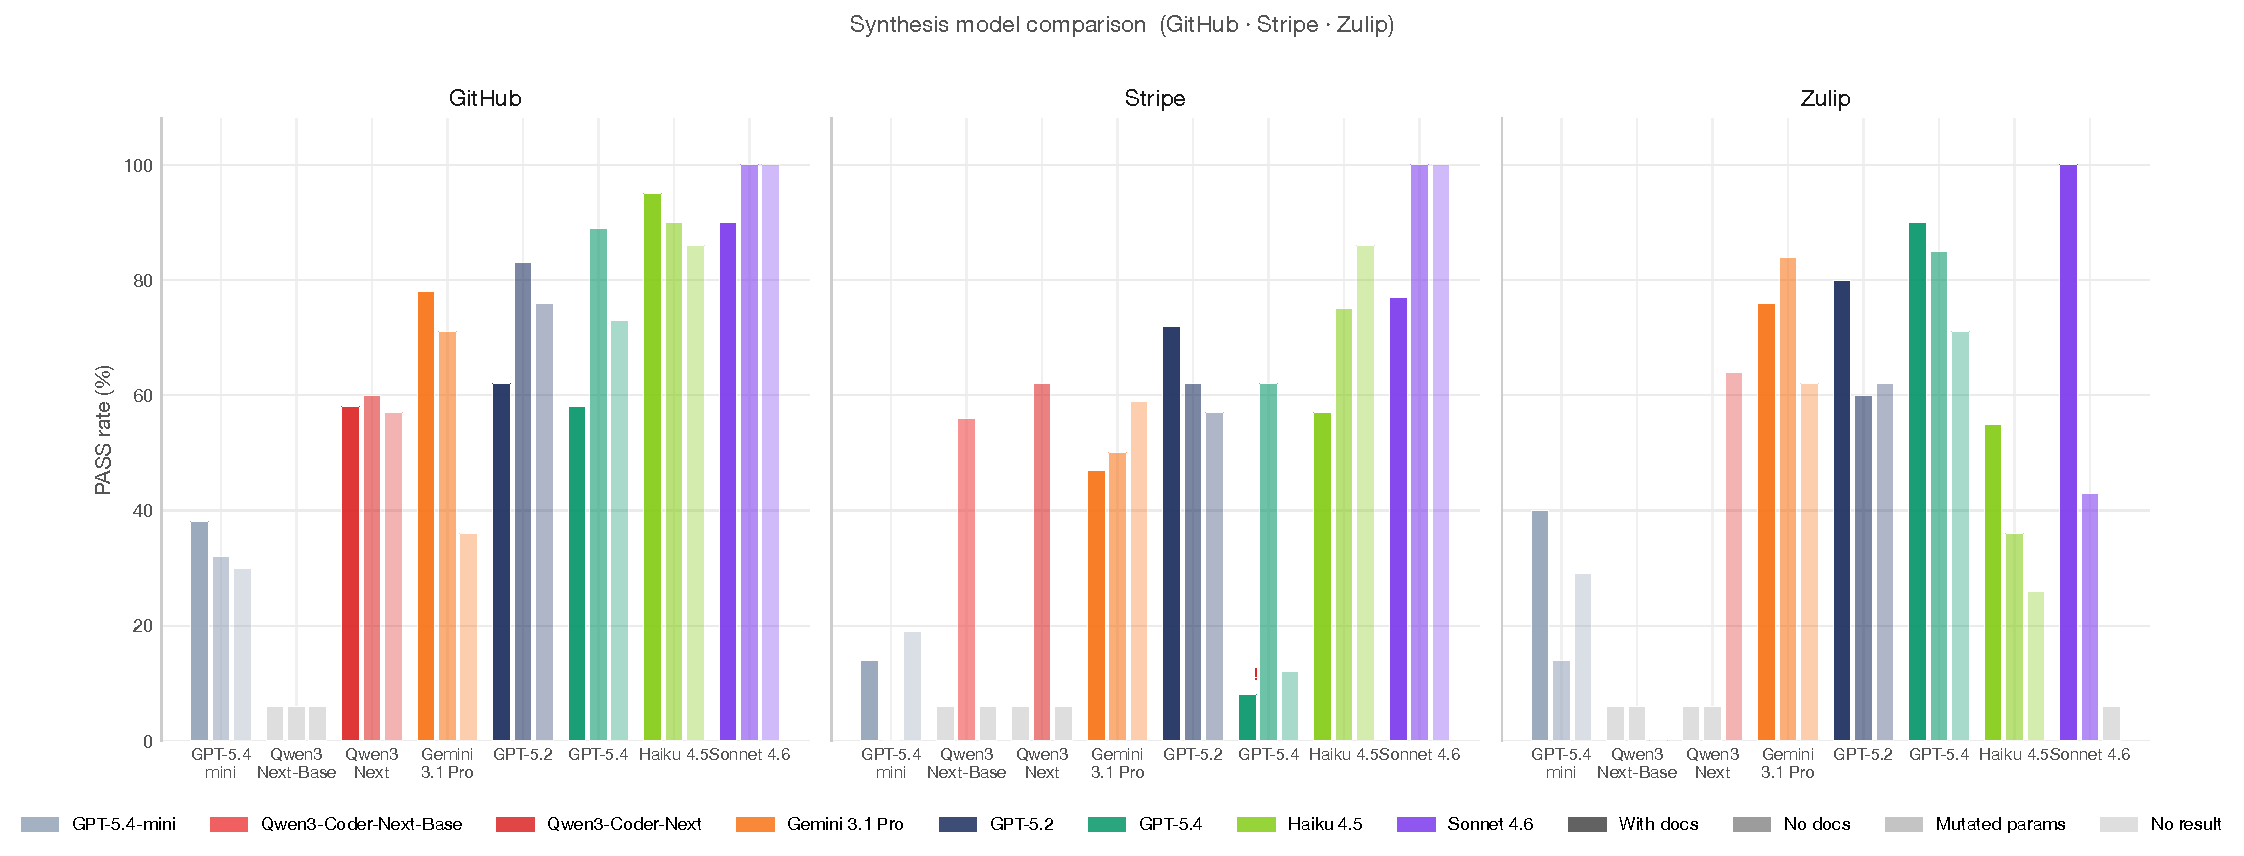
\includegraphics[width=\linewidth]{media/fig3_model_comparison.pdf}
  \caption{Per-API, per-model PASS breakdown across all synthesis conditions
    (docs, nodocs, mutated) for the common three-API set. Each group of bars
    corresponds to one API; colours distinguish synthesis models.
    Zero-height bars indicate synthesis crashes or complete tool-coverage failure.
    The GPT-5.4 Stripe docs bar (8\%) reflects broken tool stubs, not agent failure.}
  \label{fig:model_comparison}
\end{figure*}

        \chapter{Discussion}
\label{sec:discussion}
% Compare your results with the state-of-the-art and reflect upon the results and limitations of the study. You can already hint at future work to which you come back in the conclusion section.
%Write your discussion here. Do not forget to use sub-sections. Normally, the discussion starts with comparing your results to other studies as precisely as possible. The limitations should be reflected upon in terms such as reproducibility,  scalability,  generalizability,  reliability  and  validity. It is also important to mention ethical concerns.

The central finding is that automated server synthesis is a present capability, not a future prospect --- but its reliability is mediated by an underappreciated factor: whether the synthesis model's training-time representation of the target API is accurate and complete. This single axis explains the majority of variance in agent task performance across models, APIs, and documentation conditions. This chapter interprets the empirical findings in light of the research questions and prior work. Section~\ref{sec:discussion-synthesis} discusses the general feasibility of synthesis; Section~\ref{sec:discussion-gravity} examines the parametric gravity mechanism and its connection to the mechanistic probing results in Chapter~\ref{sec:mechanistic}; Section~\ref{sec:discussion-proxy} discusses SYNTH as a proxy metric; Section~\ref{sec:discussion-guidelines} derives practical guidelines for automated tool creation; and Section~\ref{sec:discussion-priorwork} positions the findings relative to prior work. Finally, key limitations are addressed in Section~\ref{sec:discussion-limitations}.

\section{Synthesis as a General Capability}
\label{sec:discussion-synthesis}

The central empirical finding is that LLM-based tool synthesis is broadly feasible: eleven of fourteen APIs achieve SYNTH $\geq 75\%$ in the docs condition, and the frontier-tier median agent pass rate of 83\% demonstrates that synthesized servers are not merely structurally valid but functionally useful. This is a non-trivial result. REST API integration involves strict interface contracts, multi-step authentication flows, and domain-specific
parameter conventions --- constraints that probabilistic generation does not inherently respect. That synthesis models navigate these requirements reliably across domains as diverse as e-commerce, communication, and financial data suggests the capability is not narrow or brittle. A five-run variance study on three APIs (Appendix~\ref{sec:apx:variance}) confirms that the no-docs condition is the most stable ($\sigma \approx 4$--$9$\,pp PASS across APIs), while the docs and mutated conditions show higher variance (up to $\sigma \approx 17$\,pp), primarily due to server size variation and degeneracy in complex APIs such as GitHub.

The two failure cases --- Jira and eBay Sell --- share a structural characteristic: extremely large documentation corpora with hundreds of endpoints distributed across deeply nested resource hierarchies. This points to a \emph{coverage scaling problem} rather than a fundamental inability to synthesize: the model understands the API but cannot attend to all endpoints
within a single synthesis context (see Appendix~\ref{sec:apx:complexity} for the relationship between documentation size and PASS). This is consistent with findings on positional bias in long contexts~\citep{liu2023lostmiddle,disentanglerecall2025},
and suggests that decomposition strategies --- synthesizing one API resource group at a time and assembling the results --- could close this gap without requiring larger context windows.

The comparison with human-authored reference servers on GitHub and Zulip sharpens this conclusion. Synthesized servers match the GitHub community server in the docs condition and substantially exceed it in the no-docs condition, while exceeding the Zulip reference in both conditions. The human references fail consistently on the same pattern: they cover the core, frequently-used API surface but omit less common but task-relevant endpoints (webhooks and Actions dispatch for GitHub; message edit and DM search for Zulip). A synthesis agent, by contrast, reads the full documentation and attempts comprehensive coverage --- and because it is not resource-constrained in the way a human contributor might be, this breadth comes without a corresponding quality trade-off.

\section{Parametric Gravity: Mechanism and Consequence}
\label{sec:discussion-gravity}

The mutation adherence results reveal a sharp split across APIs.
High-familiarity APIs (GitHub, Stripe, Shopify, Zulip, Jira) exhibit near-zero HTTP-layer adherence: the synthesis model ignores parameter mutations entirely and produces servers that reflect its training-time knowledge of the API. Low-familiarity APIs (Mastodon, Alphavantage) show near-complete adherence. This binary pattern is consistent with the training-frequency hypothesis of \citet{mallen2023knowns}: entities well-represented in pre-training data are retrieved from weights rather than from context.

The consequence for downstream performance is, however, more nuanced than a simple ``parametric reliance hurts'' narrative. For GitHub, zero adherence coincides with the highest PASS gains in the no-docs condition (+21\,pp for GPT-5.2, a single-model point estimate): the model writes from memory, and its memory is accurate. For Stripe, zero adherence coincides with a \emph{docs advantage} (+10\,pp for GPT-5.2): the model also writes from memory, but documentation provides additional signal that improves coverage. The mechanism that determines which outcome obtains is whether the synthesis model's training-time representation of the API is complete enough to be relied upon. API familiarity and API complexity interact here: GitHub is both highly familiar and structurally stable (a mature, slowly-evolving API), whereas Stripe is familiar but larger and has evolved significantly since the likely training cutoff of the primary models --- a scenario identified by \citet{lagging2025} as particularly susceptible to silent faithfulness failures. It is also worth noting that LLMs likely have strong priors for REST API patterns in general (HTTP verbs, JSON payloads, pagination conventions), even for less-exposed APIs, providing a structural scaffold that our mutation design does not directly probe.

This interpretation has a practical implication: whether to include documentation in the synthesis context is not a universal design choice but an API-specific one, and the right decision correlates with how confidently the synthesis model can write from memory. A pre-synthesis probe --- for example, asking the model to generate a list of API endpoints before providing documentation --- could serve as a low-cost signal for this confidence.

The mechanistic basis for the parametric gravity split is examined in Chapter~\ref{sec:mechanistic}. The logit-lens probing study confirms the binary pattern at the representational level: GitHub, Stripe, and eBay Commerce show 100\% parametric memory (the training-time attractor dominates within the first few transformer layers), while Mastodon, Confluence, and Jira show 100\% context-following. This early-to-mid network phenomenon aligns with feed-forward fact recall accounts~\citep{meng2022rome,factualrecall2025} and suggests that targeted context-faithful fine-tuning at transition layers could reduce parametric gravity without sacrificing synthesis capability. The finding also has implications for model choice: instruction fine-tuning and RLHF alter the geometry of the residual stream~\citep{posttrainingreshapes2025}, which may help explain the wide spread in adherence rates observed in Chapter~\ref{sec:results} --- GPT-5.4, for instance, reaches near-complete adherence on Confluence and eBay Commerce, while Gemini~3.1~Pro shows near-zero adherence across the benchmark, despite being large-scale models with comparable pre-training exposure (Gemini~3.1~Pro is classified as mid-tier in our benchmark based on synthesis reliability rather than raw model scale).

\section{Synthesis Quality as a Proxy Metric}
\label{sec:discussion-proxy}

The strong SYNTH--PASS correlation ($r = 0.937$, $p < 0.0001$, $n = 209$ across all synthesis models) has a direct practical implication: synthesis sufficiency --- assessed by an LLM judge examining the server's tool list without running the evaluation agent --- is a reliable predictor of downstream agent task performance. A judge sensitivity study across four models (Appendix~\ref{sec:apx:judge}) confirms that SYNTH scores are stable across judges: Gemini~3~Flash and GPT-4.1 agree within $\pm$12\,pp on the majority of conditions, validating the judge-based metric design. This matters because the full evaluation pipeline --- spinning up a sandboxed API environment, running the evaluation agent for up to 15 turns per task, calling the judge --- is expensive in both API quota and wall time. SYNTH can be assessed at synthesis time, before any agent evaluation occurs.

The two regimes visible in Figure~\ref{fig:scatter} sharpen when this metric is used diagnostically. For synthesis-limited cases (low SYNTH, low PASS), investment in improving synthesis quality --- better documentation pre-processing, larger context windows, iterative tool refinement --- will directly improve agent outcomes. For agent-limited cases (high SYNTH, lower PASS), the bottleneck is the evaluation agent's ability to compose available tools into correct multi-step plans, and improving synthesis will not help; the intervention should target the agent's reasoning or task decomposition.

One class of outlier is worth noting: Spoonacular in the docs condition achieves PASS=100\% despite SYNTH=75\%. This occurs because the evaluation agent compensates for minor coverage gaps using general culinary knowledge to reformulate queries through available tools. This agent-compensation effect is bounded --- it requires the agent to have its own parametric knowledge about the domain --- and cannot be relied upon for APIs in unfamiliar domains (compare Jira, where the agent has no comparable domain model to fall back on).

\section{Practical Design Guidelines}
\label{sec:discussion-guidelines}

The results point to several concrete recommendations for practitioners building full-server MCP synthesis pipelines --- systems that must produce complete, protocol-compliant tool servers rather than individual function stubs.

\paragraph{Documentation pre-processing matters for large APIs.}
For APIs with more than approximately 50 endpoints, raw documentation dumps produce coverage gaps: the synthesizer cannot attend to all endpoints in a single pass. Structured chunking by resource group, with per-chunk synthesis followed by assembly, is likely to produce higher SYNTH scores than end-to-end synthesis from a monolithic documentation corpus.

\paragraph{Omitting documentation is safe only for mature, well-known APIs.} For APIs with saturation-level representation in model training data --- GitHub, Mastodon, and major productivity platforms such as Notion --- the no-docs condition matches or exceeds the docs condition. This effect is partly about familiarity and partly about API maturity: the APIs where no-docs succeeds tend to be stable, slowly-evolving interfaces with few breaking version changes, so the model's training-time memory remains accurate. Documentation can add noise by providing competing context that the model must adjudicate against its priors, particularly for long, partially-outdated documentation files. For APIs at intermediate familiarity or with more active versioning (Stripe, Zulip), documentation provides a net benefit, and omitting it degrades performance. Practitioners should consider a pre-synthesis familiarity check --- for instance, asking the model to list API endpoints before receiving documentation --- before deciding whether to include documentation in the synthesis context.

\paragraph{Grounding manifests provide a weak but useful quality signal.} Requiring the synthesizer to produce a \texttt{grounding.json} enables a fast post-synthesis check: verify that every tool is anchored to an existing documentation file and a syntactically valid endpoint string. This does not guarantee implementation correctness --- a model can cite the right document while misreading it --- but tools lacking any documentation anchor are a reliable signal of unconstrained parametric generation, and missing grounding coverage (tools with no entry) often correlates with structural synthesis failures.

\paragraph{SYNTH is a cheap pre-flight metric.}
Running an LLM judge over the tool list before committing to full agent evaluation identifies synthesis-limited cases early. A SYNTH threshold of around 75\% appears to be the boundary below which full evaluation is unlikely to produce acceptable PASS rates in our benchmark; APIs below this threshold benefit more from re-synthesis than from agent tuning.

\paragraph{Prefer models with strong context-faithfulness for evolving or versioned APIs.} When the target API is less familiar to the model, or when documentation has been deliberately structured to override training priors, synthesis models that exhibit higher context adherence --- GPT-5.4 in our comparison, which reaches near-complete adherence on several mid-familiarity APIs --- produce more reliable servers. The GPT-5.4 regression on Stripe (8\% vs.\ 72\% baseline) illustrates the risk of deploying a model with strong parametric priors on an API that has evolved significantly since its training cutoff.

\paragraph{Looking ahead.} The guidelines above are grounded in the current single-agent synthesis scaffold. Future system designs could push further: neuro-symbolic verification (type-checking schemas against an API registry before committing), multi-agent pipelines with planner/verifier/assembler separation, and adaptive documentation inclusion (gated by a pre-synthesis familiarity probe) are natural extensions that the benchmark motivates but does not evaluate. These directions are discussed in the conclusion.

\section{Comparison with Prior Work}
\label{sec:discussion-priorwork}

Direct numerical comparison with prior work is complicated by the absence of overlapping evaluation sets: ToolFactory~\citep{toolfactory2025} and Doc2Agent~\citep{doc2agent2025} each evaluate on their own API selections and do not report PASS rates on the same 14 APIs used here. Qualitative comparison is nonetheless informative.

ToolFactory targets OpenAPI-specified inputs and focuses on coverage of the formal schema; our benchmark uses raw Markdown documentation, a substantially harder input modality that better reflects real practitioner conditions. Where ToolFactory reports synthesis success in terms of schema coverage, we report end-to-end agent task completion, which additionally exercises tool naming, description quality, and implementation correctness under live API execution.

Doc2Agent is closest to our work in motivation: it demonstrates that callable tool implementations can be generated from documentation at scale across many APIs. However, Doc2Agent generates individual tool stubs, not complete deployable servers; our synthesis target is a full MCP server with authentication, multi-tool coordination, and protocol compliance --- a more demanding integration target that is evaluated end-to-end through live API execution. Our benchmark additionally adds the no-docs and mutated conditions that Doc2Agent does not evaluate, enabling the parametric knowledge analysis that is our primary empirical contribution, and our comparison against the GitHub and Zulip community servers provides evidence on whether synthesized servers can match or exceed human-authored alternatives.

WAPIIBench~\citep{wapiibench2025} catalogues LLM-generated API integration errors against live services and reports error taxonomies that partially overlap with our failure cause categories (\verdict{tool\_schema}, \verdict{tool\_implementation}). Their finding that authentication and parameter serialisation errors are the most frequent failure types reflects a different primary failure regime than ours: WAPIIBench evaluates individual API calls, where the tool exists but its implementation is incorrect. Our primary failure mode is \verdict{tool\_coverage} --- the required tool was never synthesized at all --- so that when a tool is present, our \verdict{tool\_implementation} and \verdict{tool\_schema} rates are relatively low. This difference illustrates how full-server synthesis introduces a distinct and earlier failure point not captured by single-call evaluation.

\section{Limitations}
\label{sec:discussion-limitations}

\paragraph{Generalizability.}
The 14-API evaluation set spans five domains and a wide range of API sizes, but is not exhaustive. All selected APIs are REST-based, return JSON, and have English-language documentation. APIs with non-REST interfaces (GraphQL, gRPC), streaming responses, complex webhook architectures, or non-English documentation are not represented. The degree to which the parametric gravity findings generalise to programming-language SDKs rather than HTTP APIs is also unknown: the mutation adherence analysis is specific to the HTTP parameter-name setting.

\paragraph{Reliability.}
PASS rates are determined by an LLM judge, which introduces variability. We use a fixed judge model (Gemini~3~Flash) with a structured fixed-format prompt to reduce inconsistency. A judge sensitivity study across four judge models is reported in Appendix~\ref{sec:apx:judge} (Table~\ref{tab:apx:judge}); Gemini~3~Flash agrees with GPT-4.1 within $\pm$12\,pp on the majority of conditions. Similarly, the probing analysis rests on a single open-weight model; results should not be taken as established fact about frontier-scale models.

\paragraph{Reproducibility.}
All synthesis runs are stochastic: the same synthesis model and documentation may produce a different server on a different run. We report single-run results per condition rather than averages over multiple runs, which means some variance in PASS and SYNTH is unaccounted for; a synthesis variance study across five repeated runs on three APIs is reported in Appendix~\ref{sec:apx:variance} (Table~\ref{tab:apx:var_summary}). API sandboxes may also change state between runs, introducing noise in write-task evaluations.

\paragraph{Ethical considerations.}
Automated tool synthesis lowers the barrier to creating API integrations, including potentially for APIs whose terms of service restrict automated access or data extraction. The benchmark deliberately uses official sandbox environments with test credentials, but production deployment of synthesis pipelines against APIs not designed for automated access raises terms-of-service (ToS) and privacy concerns that practitioners should assess case by case. There is also an energy cost to running large synthesis models at scale; the no-docs condition, which is substantially cheaper, may be preferable where API familiarity is high, reducing unnecessary compute.
        \chapter{Conclusion}
\label{sec:conclusion}
% Answer each research question and address how the limitations of the study qualify the conclusion.
%Write your conclusion here. Be sure that the relation between the research gap and your contribution is clear. Be honest about how limitations in the study qualify the answer on the research question.


This thesis addressed a gap in the tool-use literature: the assumption that
tools are given. We asked whether language models can synthesize functional
API tool servers from documentation, whether those servers enable effective
agent task completion, and what role parametric knowledge plays in both.
Below we answer each research question and qualify the answers with the
relevant limitations of the study.

\paragraph{RQ1: Can LLMs synthesize functional API tool servers from documentation alone?}
Yes, for most APIs tested. Eleven of fourteen APIs achieve SYNTH $\geq 75\%$ in the docs condition, and the frontier-tier median PASS of 83\% demonstrates these servers are not just syntactically valid but produce real task-completion utility in practice. The dominant failure mode is coverage gap (omitted endpoints) rather than structural failure (broken or non-executable servers). Notably, successful synthesis does not require frontier-scale models for all APIs: mid-tier models achieve competitive PASS on simpler, high-familiarity APIs (e.g., GitHub, Mastodon), though frontier models produce more reliable and consistent coverage across the full benchmark. This answer is qualified by generalizability: all APIs in the benchmark are REST-based with English documentation, and synthesis feasibility for larger or differently structured APIs remains to be established.

\paragraph{RQ2: Do synthesized servers enable effective agent task completion, compared to human-authored references?}
Yes, at a frontier-tier median PASS of 83\% in the docs condition, and synthesized servers match or exceed the two available human-authored references. On GitHub, no-docs synthesis achieves 83\% PASS (81--90\% across variance-study runs) against an official server baseline of 65\%; on Zulip, docs-condition synthesis scores 80\% against a baseline of 68\%. The qualification in this case is that agent performance is partially
confounded by the fixed evaluation agent (Gemini~2.5~Pro); agent-limited failures identified in our benchmark may not reflect the same limitations with a different evaluator.

\paragraph{RQ3: To what extent do synthesizers rely on parametric knowledge, and does this affect performance?}
Substantially, and in a way that is API-dependent. High-familiarity APIs show near-zero HTTP mutation adherence, indicating synthesis models write almost entirely from memory. The performance consequence is non-monotonic: parametric reliance helps on GitHub (where model memory is accurate and complete) but does not on Stripe (where documentation provides additional coverage). This answer is limited by the fact that adherence is measured for a fixed set of 4--6 mutated parameters per API; the pattern may differ for other models or mutation strategies.

\paragraph{RQ4: How does documentation availability affect synthesis and agent performance?}
The aggregate effect is smaller than expected: the no-docs condition median (88\%) meets or exceeds the docs condition median (83\%), driven by high-familiarity APIs where model memory substitutes for documentation. Documentation helps for less familiar or more complex APIs (Stripe, Zulip) and hurts for highly familiar or simply-structured ones (GitHub, Mastodon), suggesting the effect is mediated by training coverage rather than documentation quality per se. This finding
is subject to the static-snapshot limitation: documentation was scraped at a single point in time, and results may differ for documentation that is more consistently current or higher quality.

\paragraph{RQ5: Does synthesis quality predict agent task performance?}
Strongly: $r = 0.937$ ($p < 0.0001$, $n = 209$ across all models). SYNTH, assessable without running the evaluation agent, is a reliable proxy for PASS. This holds across APIs and conditions, with the main exceptions being cases where the
evaluation agent compensates for synthesis gaps using its own domain knowledge (Spoonacular) or where the agent fails despite sufficient tools (agent-limited cases). The correlation is measured on our 14-API benchmark; whether it holds at this strength for a wider or different API distribution is unknown.

\section*{Research Gap and Contribution}

Prior work treats the tool layer as given. We have shown that synthesizing it automatically is feasible today for most practically relevant REST APIs, and that the primary bottleneck for large APIs is context-window coverage of documentation rather than a fundamental capability limit. The key novelty is the synthesis \emph{target}: a complete, protocol-compliant MCP server rather than individual tool stubs, which is what enables genuine end-to-end evaluation through live API execution. The SYNTH metric and the controlled ablation design --- isolating parametric knowledge from documentation grounding --- are methodological contributions that generalise beyond this benchmark to any evaluation of documentation-grounded
code generation. A preliminary mechanistic analysis (Chapter~\ref{sec:mechanistic}) grounds the parametric gravity phenomenon in transformer representations, connecting behavioural findings to the interpretability literature.

\section*{Future Work}

Several directions emerge directly from the findings.

\textbf{Coverage scaling.} The most immediate target is decomposed synthesis for large APIs (Jira, eBay Sell): synthesizing one resource group at a time and assembling the result addresses the context-window bottleneck without requiring larger models.

\textbf{Proprietary and non-public APIs.} All 14 benchmark APIs have public documentation. Extending synthesis to internal or proprietary APIs --- where documentation may be incomplete, inconsistently maintained, or confidential --- introduces new challenges around grounding signal quality and access control that merit separate investigation.

\textbf{Neuro-symbolic and constraint-driven synthesis.} A natural follow-on to the full-server setting is to enforce protocol constraints symbolically at synthesis time: type-checking tool schemas, validating endpoint paths against an API registry, or running a lightweight stub call before committing to an implementation. Such neuro-symbolic approaches could eliminate the most common \verdict{tool\_schema} failures without requiring re-synthesis.

\textbf{Adaptive documentation inclusion.} Our findings suggest that the optimal synthesis context is API-specific and predictable from familiarity. A practical system could automate this decision: a pre-synthesis probe (or mutation adherence mini-run) could estimate model confidence in the API's parametric representation and gate documentation inclusion accordingly.

\textbf{Specialised multi-agent synthesis pipelines.} The single-agent synthesis scaffold used here is minimal by design. More capable pipelines could include a planner that decomposes synthesis by resource group, a verifier that tests generated tools against the live API, and an assembler that merges partial servers --- analogous to specialised coding agents for software engineering tasks.

\textbf{Live versioning benchmarks.} Extending the probing analysis to frontier-scale open-weight models would test whether the layer-transition pattern generalises. A live benchmark that re-runs synthesis as APIs evolve would capture the dynamic challenge that static snapshots cannot, particularly for APIs at the Stripe/Zulip familiarity tier where parametric memory and documentation are in active tension.


\bibliographystyle{ACM-Reference-Format}
\bibliography{bibliographies/references}

% \newpage
\appendix
        % You can choose whether you prefer a single or double column appendix.
% Whatever you choose, you will need to stick to it throughout the appendix.
\onecolumn

\chapter{Supplementary Results}
\label{sec:apx:first_appendix}

% ------------------------------------------------------------
\section{Full Per-Model Results Table}
\label{sec:apx:full_results}
% ------------------------------------------------------------

Table~\ref{tab:apx:full_results} reports PASS (\%) for every synthesis model, API, and condition evaluated in this thesis. Models that failed to produce a runnable server are recorded as 0\%. ``---'' indicates the condition was never attempted. GPT-4.1, Gemini~2.5 Pro, and Gemini~3.5 Flash produced no valid servers across any condition and are omitted; their failure modes are documented in Section~\ref{sec:methodology}. Alphavantage results for Sonnet~4.6 and Haiku~4.5 are omitted due to API rate-limit exhaustion during evaluation (ENVIRONMENT errors on all tasks).

\begin{table}[htbp]
  \centering
  \caption{Agent PASS (\%) across all synthesis models, APIs, and conditions.
    0 = synthesis crash or complete tool-coverage failure.
    \colorbox{red!12}{Red} = below 50\%. --- = not evaluated.
    D = docs, N = nodocs, M = mutated.}
  \label{tab:apx:full_results}
  \setlength{\tabcolsep}{3pt}
  \scriptsize
  \begin{tabular}{l rrr rrr rrr rrr rrr rrr rrr rrr}
    \toprule
    & \multicolumn{3}{c}{\textbf{GPT-5.4-mini}}
    & \multicolumn{3}{c}{\textbf{Qwen3-Next-Base}}
    & \multicolumn{3}{c}{\textbf{Qwen3-Next}}
    & \multicolumn{3}{c}{\textbf{Gem~3.1 Pro}}
    & \multicolumn{3}{c}{\textbf{GPT-5.2}}
    & \multicolumn{3}{c}{\textbf{GPT-5.4}}
    & \multicolumn{3}{c}{\textbf{Haiku~4.5}}
    & \multicolumn{3}{c}{\textbf{Sonnet~4.6}} \\
    \cmidrule(lr){2-4}\cmidrule(lr){5-7}\cmidrule(lr){8-10}\cmidrule(lr){11-13}
    \cmidrule(lr){14-16}\cmidrule(lr){17-19}\cmidrule(lr){20-22}\cmidrule(lr){23-25}
    \textbf{API} & D & N & M & D & N & M & D & N & M & D & N & M & D & N & M & D & N & M & D & N & M & D & N & M \\
    \midrule
    GitHub         & \cellcolor{red!12}38 & \cellcolor{red!12}32 & \cellcolor{red!12}30 & \cellcolor{red!12}0 & \cellcolor{red!12}0 & \cellcolor{red!12}0 & 58 & 60 & 57 & 78 & 71 & \cellcolor{red!12}36 & 62 & 83 & 76 & 58 & 89 & 73 & 95 & 90 & 86 & 90 & 100 & 100 \\
    Stripe         & \cellcolor{red!12}14 & \cellcolor{red!12}0 & \cellcolor{red!12}19 & \cellcolor{red!12}0 & 56 & \cellcolor{red!12}0 & \cellcolor{red!12}0 & 62 & \cellcolor{red!12}0 & \cellcolor{red!12}47 & 50 & 59 & 72 & 62 & 57 & \cellcolor{red!12}8 & 62 & \cellcolor{red!12}12 & 57 & 75 & 86 & 77 & 100 & 100 \\
    Zulip          & \cellcolor{red!12}40 & \cellcolor{red!12}14 & \cellcolor{red!12}29 & \cellcolor{red!12}0 & \cellcolor{red!12}0 & \cellcolor{red!12}0 & \cellcolor{red!12}0 & \cellcolor{red!12}0 & 64 & 76 & 84 & 62 & 80 & 60 & 62 & 90 & 85 & 71 & 55 & \cellcolor{red!12}36 & \cellcolor{red!12}26 & 100 & \cellcolor{red!12}43 & \cellcolor{red!12}0 \\
    \midrule
    Alphavantage   & --- & --- & --- & 92 & --- & --- & --- & --- & --- & 100 & 100 & 90 & 86 & 90 & 88 & 80 & 92 & 78 & ---$^a$ & ---$^a$ & ---$^a$ & ---$^a$ & ---$^a$ & ---$^a$ \\
    Confluence     & 83$^b$ & \cellcolor{red!12}40$^b$ & \cellcolor{red!12}0 & 64 & --- & --- & \cellcolor{red!12}39 & 100$^c$ & 50 & \cellcolor{red!12}0 & 100 & 100 & 92 & 93 & 91 & 69 & 100 & 85 & 80 & \cellcolor{red!12}33 & \cellcolor{red!12}33 & \cellcolor{red!12}0 & 94 & \cellcolor{red!12}47 \\
    eBay Buy       & --- & --- & --- & \cellcolor{red!12}6 & --- & --- & \cellcolor{red!12}12 & 80 & \cellcolor{red!12}6 & 90 & 67 & \cellcolor{red!12}0 & 73 & 67 & 80 & 69 & 92 & 100 & 80 & 67 & 100 & \cellcolor{red!12}0 & 79 & \cellcolor{red!12}33 \\
    eBay Commerce  & --- & --- & --- & \cellcolor{red!12}45 & --- & --- & 100 & \cellcolor{red!12}0 & \cellcolor{red!12}11 & 83 & \cellcolor{red!12}44 & \cellcolor{red!12}45 & 100 & 89 & 55 & 88 & \cellcolor{red!12}40 & 62 & \cellcolor{red!12}30 & \cellcolor{red!12}10 & 50 & 100 & \cellcolor{red!12}0 & --- \\
    eBay Sell      & --- & --- & --- & --- & \cellcolor{red!12}0 & --- & 100$^c$ & \cellcolor{red!12}0 & \cellcolor{red!12}0 & \cellcolor{red!12}38 & \cellcolor{red!12}8 & \cellcolor{red!12}23 & \cellcolor{red!12}38 & 50 & \cellcolor{red!12}43 & \cellcolor{red!12}29 & \cellcolor{red!12}45 & \cellcolor{red!12}44 & \cellcolor{red!12}17 & \cellcolor{red!12}9 & \cellcolor{red!12}36 & \cellcolor{red!12}0 & 73 & --- \\
    Jira           & --- & --- & --- & --- & --- & --- & 71 & \cellcolor{red!12}0 & \cellcolor{red!12}42 & 58 & \cellcolor{red!12}44 & \cellcolor{red!12}31 & 50 & \cellcolor{red!12}25 & 50 & 57 & 50 & 57 & 62 & \cellcolor{red!12}7 & 64 & 73 & 58 & 79 \\
    Mastodon       & --- & --- & --- & \cellcolor{red!12}0 & --- & \cellcolor{red!12}0 & 87 & 80 & 54 & 100 & 92 & 87 & 100 & 100 & 100 & 91 & 90 & 100 & 93 & \cellcolor{red!12}40 & 86 & \cellcolor{red!12}0 & \cellcolor{red!12}0 & 92 \\
    Notion         & --- & --- & --- & --- & \cellcolor{red!12}0 & --- & 69 & \cellcolor{red!12}5 & \cellcolor{red!12}0 & 94 & 94 & 100 & 78 & 100 & 100 & 62 & 100 & \cellcolor{red!12}0 & 56 & \cellcolor{red!12}5 & 50 & 100 & 87 & 85 \\
    OpenWeatherMap & --- & --- & --- & --- & --- & --- & 100 & 86 & 100 & 85 & 90 & 95 & 100 & 86 & 100 & 100 & 95 & 100 & 95 & 65 & 60 & \cellcolor{red!12}0 & 100 & \cellcolor{red!12}0 \\
    Shopify        & --- & --- & --- & --- & \cellcolor{red!12}0 & \cellcolor{red!12}0 & 94 & 82 & 67 & 80 & 70 & 93 & 87 & 92 & 62 & 83 & 92 & 53 & 93 & 75 & 94 & 100 & \cellcolor{red!12}0 & --- \\
    Spoonacular    & --- & --- & --- & --- & 60 & --- & --- & --- & --- & 83 & 91 & 90 & 100 & 90 & 78 & 80 & 82 & 60 & ---$^d$ & 79 & 86 & 93 & \cellcolor{red!12}0 & 92 \\
    \bottomrule
  \end{tabular}
  \par\smallskip
  \raggedright\scriptsize
  Qwen3-Next-Base = Qwen3-Coder-Next-Base; Qwen3-Next = Qwen3-Coder-Next.
  $^a$ Rate-limited; shared 25\,req/day key exhausted.
  $^b$ GPT-5.4-mini full matrix aborted after 26/112 evals; only confluence nodocs/mutated returned non-zero.
  $^c$ Tiny scoreable N ($\leq$3 due to ENVIRONMENT errors); treat with caution.
  $^d$ Haiku spoonacular docs pending at time of writing.
\end{table}

\begin{table}[htbp]
  \centering
  \caption{PASS and SYNTH (\%) for the no-docs and mutated conditions, GPT-5.2 reference model.
    Rows in the same order as Table~\ref{tab:pass_results}.
    \colorbox{red!12}{Red} = PASS below 50\%.
    SYNTH = server synthesis sufficiency (fraction of task-relevant tools present).}
  \label{tab:apx:nodocs_mutated}
  \setlength{\tabcolsep}{5pt}
  \small
  \begin{tabular}{l rr rr}
    \toprule
    & \multicolumn{2}{c}{\textbf{No-docs}} & \multicolumn{2}{c}{\textbf{Mutated}} \\
    \cmidrule(lr){2-3}\cmidrule(lr){4-5}
    \textbf{API} & \textbf{PASS} & \textbf{SYNTH} & \textbf{PASS} & \textbf{SYNTH} \\
    \midrule
    OpenWeatherMap & 86  & 83  & 100 & 100 \\
    eBay Commerce  & 89  & 85  & 55  &  54 \\
    Mastodon       & 100 & 100 & 100 & 100 \\
    Zulip          & 60  &  48 &  62 &  64 \\
    Spoonacular    & 90  &  75 &  78 &  75 \\
    Shopify        & 92  &  94 &  62 &  61 \\
    Alphavantage   & 90  &  89 &  88 &  89 \\
    Confluence     & 93  &  95 &  91 &  95 \\
    Notion         & 100 & 100 & 100 & 100 \\
    eBay Buy       & 67  &  94 &  80 &  88 \\
    GitHub         & 83  &  87 &  76 &  61 \\
    Jira           & \cellcolor{red!12}25 & 44 & \cellcolor{red!12}50 & 56 \\
    Stripe         & 62  &  68 &  57 &  73 \\
    eBay Sell      & \cellcolor{red!12}50 & 50 & \cellcolor{red!12}43 & 43 \\
    \midrule
    \textit{Median} & \textit{88} & \textit{86} & \textit{77} & \textit{75} \\
    \bottomrule
  \end{tabular}
\end{table}

% ------------------------------------------------------------
\section{Synthesis Variance Study}
\label{sec:apx:variance}
% ------------------------------------------------------------

To quantify synthesis stochasticity, we ran GPT-5.2 five times on each of three APIs and all three conditions, holding all other variables fixed. Tables~\ref{tab:apx:var_shopify}--\ref{tab:apx:var_github} report per-run PASS and SYNTH; Table~\ref{tab:apx:var_summary} summarises key statistics.

\paragraph{Shopify.}
The nodocs condition is the most stable (Table~\ref{tab:apx:var_shopify_nd}): SYNTH locks at 94\% on every run ($\sigma=0$), and CURRENT ranges 80--94\% (mean 90\%, $\sigma\approx6$\,pp). Docs condition is high-variance (Table~\ref{tab:apx:var_shopify_d}): CURRENT 59--93\% ($\sigma\approx13$\,pp), with no degeneracy but large differences between small (131-line, 93\%) and large (538-line, 75\%) servers. Mutated (Table~\ref{tab:apx:var_shopify_m}) has one startup crash and CURRENT 67--92\% across non-crash runs; mutation adherence is perfectly stable (0\% HTTP / 20\% iface on every run).

\begin{table}[htbp]
  \centering
  \caption{Shopify docs variance (5 runs, GPT-5.2). Lines = server.py line count.}
  \label{tab:apx:var_shopify_d}
  \small
  \begin{tabular}{lrrrr}
    \toprule
    Run & Lines & PASS & SYNTH & Notes \\
    \midrule
    Reference & 552 & 87\% & 89\% & — \\
    1 & 131 & 93\% & 94\% & — \\
    2 & 143 & 93\% & 94\% & Optional (discounts only) \\
    3 & 522 & 79\% & 83\% & — \\
    4 & 538 & 75\% & 83\% & — \\
    5 & 112 & 59\% & 61\% & — \\
    \midrule
    \multicolumn{2}{l}{Range} & 59--93\% & 61--94\% & $\sigma$(PASS)$\approx$13\,pp \\
    \bottomrule
  \end{tabular}
\end{table}

\begin{table}[htbp]
  \centering
  \caption{Shopify nodocs variance (5 runs, GPT-5.2).}
  \label{tab:apx:var_shopify_nd}
  \small
  \begin{tabular}{lrrrr}
    \toprule
    Run & Lines & PASS & SYNTH & Notes \\
    \midrule
    Reference & large & 92\% & 94\% & — \\
    1 & 186 & 92\% & 94\% & — \\
    2 & 230 & 94\% & 94\% & — \\
    3 & 109 & 93\% & 94\% & — \\
    4 & 115 & 80\% & 94\% & — \\
    5 & 151 & 93\% & 94\% & VPN drop re-run \\
    \midrule
    \multicolumn{2}{l}{Range} & 80--94\% & 94\% & $\sigma$(SYNTH)=0 \\
    \bottomrule
  \end{tabular}
\end{table}

\begin{table}[htbp]
  \centering
  \caption{Shopify mutated variance (5 runs, GPT-5.2, patched). HTTP~Adh / Iface~Adh stable across all runs.}
  \label{tab:apx:var_shopify_m}
  \small
  \begin{tabular}{lrrrr}
    \toprule
    Run & Lines & PASS & SYNTH & HTTP / Iface \\
    \midrule
    Reference & large & 62\% & 61\% & 0\% / 20\% \\
    1 & 142 & 67\% & 72\% & 0\% / 20\% \\
    2 & 121 & 0\% (crash) & --- & 0\% / 20\% \\
    3 & 172 & 92\% & 94\% & 0\% / 20\% \\
    4 & 174 & 80\% & 83\% & 0\% / 20\% \\
    5 & 134 & 79\% & 83\% & 0\% / 20\% \\
    \midrule
    \multicolumn{2}{l}{Range (excl.\ crash)} & 67--92\% & 72--94\% & $\sigma$(adh)=0 \\
    \bottomrule
  \end{tabular}
\end{table}

\paragraph{GitHub.}
Docs synthesis is highly degenerate (Table~\ref{tab:apx:var_github}): 4 of 6 runs produce stub servers with 1--5 tools instead of the 46--61 tools in valid runs. Valid runs score 62--67\%, tight with the human MCP reference (65\%). Nodocs degeneracy rate drops to 0/3; all runs outperform the reference (81--90\%). Mutated is universally degenerate (7/7 runs, 0--6 tools); the mutation context consistently destabilises GitHub synthesis for this model.

\begin{table}[htbp]
  \centering
  \caption{GitHub docs variance (6 runs) and nodocs variance (3 runs). Human reference shown for comparison.}
  \label{tab:apx:var_github}
  \small
  \begin{tabular}{llrrrl}
    \toprule
    Cond & Run & Tools & PASS & SYNTH & Status \\
    \midrule
    — & Human ref & — & 65\% & 65\% & — \\
    \midrule
    docs & Reference & 53 & 62\% & 61\% & — \\
    docs & 1 & 46 & 67\% & 70\% & — \\
    docs & 2 & 2 & --- & --- & Degenerate \\
    docs & 3 & 3 & --- & --- & Degenerate \\
    docs & 4 & 5 & 0\% & --- & Degenerate \\
    docs & 5 & 61 & 64\% & 57\% & — \\
    docs & 6 & 1 & --- & --- & Degenerate \\
    \midrule
    nodocs & Reference & — & 83\% & 87\% & — \\
    nodocs & 1 & 63 & 86\% & 87\% & — \\
    nodocs & 2 & 61 & 90\% & 91\% & — \\
    nodocs & 3 & 63 & 81\% & 83\% & — \\
    \bottomrule
  \end{tabular}
\end{table}

\paragraph{Stripe.}
Docs and nodocs each have 1/5 degeneracy (startup crash). Valid docs runs score 46--67\% (ref 72\%); the bottleneck is AGENT\_REASONING (8--14 failures per run), not tool coverage. Nodocs valid runs score 38--62\% (ref 62\%), with lower SYNTH (57--73\%) reflecting weaker parametric knowledge of Stripe's API surface. Mutated shows the widest variance (20--69\% across 4 non-degenerate runs); adherence itself varies run-to-run (0--20\% HTTP), in contrast to Shopify's perfectly stable adherence.

\begin{table}[htbp]
  \centering
  \caption{Stripe variance summary across all three conditions (5 runs each, GPT-5.2).}
  \label{tab:apx:var_stripe}
  \small
  \begin{tabular}{lrrrl}
    \toprule
    Condition & PASS range & SYNTH range & Degeneracy & Bottleneck \\
    \midrule
    docs & 46--67\% & 68--77\% & 1/5 (crash) & AGENT\_REASONING \\
    nodocs & 38--62\% & 57--73\% & 1/5 (crash) & TOOL\_COVERAGE \\
    mutated & 20--69\% & 45--77\% & 1/5 (crash) & Mixed \\
    \bottomrule
  \end{tabular}
\end{table}

\begin{table}[htbp]
  \centering
  \caption{Variance summary statistics across all APIs and conditions. Nodocs is the most
    reliable condition; docs and mutated show higher variance and degeneracy.}
  \label{tab:apx:var_summary}
  \small
  \begin{tabular}{lrrl}
    \toprule
    Condition & PASS $\sigma$ (mean) & Degeneracy rate & Primary failure mode \\
    \midrule
    Shopify docs    & $\approx$13\,pp & 0/5  & Server size variance \\
    Shopify nodocs  & $\approx$6\,pp  & 0/5  & Stable (SYNTH fixed) \\
    Shopify mutated & $\approx$11\,pp & 1/5  & Crash, adherence stable \\
    GitHub docs     & high    & 4/6  & Degenerate stubs \\
    GitHub nodocs   & $\approx$4\,pp  & 0/3  & Stable, beats reference \\
    GitHub mutated  & ---     & 7/7  & Universal degeneracy \\
    Stripe docs     & $\approx$9\,pp  & 1/5  & AGENT\_REASONING \\
    Stripe nodocs   & $\approx$9\,pp  & 1/5  & TOOL\_COVERAGE \\
    Stripe mutated  & $\approx$17\,pp & 1/5  & Adherence variance \\
    \bottomrule
  \end{tabular}
\end{table}

% ------------------------------------------------------------
\section{Judge Sensitivity Study}
\label{sec:apx:judge}
% ------------------------------------------------------------

To assess whether results depend on the choice of judge model, we re-ran evaluation of five APIs under all three conditions using four different judge LLMs while holding the synthesis server and agent run fixed. Table~\ref{tab:apx:judge} reports per-judge PASS; Table~\ref{tab:apx:judge_summary} summarises key patterns.

\begin{table}[htbp]
  \centering
  \caption{Judge sensitivity study: PASS (\%) per judge model across 5 APIs and 3 conditions.
    AR = AGENT\_REASONING undefined count (high AR = judge over-classifies agent answers as incomplete).
    Baseline judge is Gemini~3~Flash.}
  \label{tab:apx:judge}
  \small
  \setlength{\tabcolsep}{4pt}
  \begin{tabular}{llrrrr}
    \toprule
    \textbf{API} & \textbf{Cond} & \textbf{Gem~3~Flash} & \textbf{GPT-4.1} & \textbf{GPT-5.4-mini} & \textbf{Gem~2.5~Flash} \\
    \midrule
    GitHub & docs    & 62\% (AR=2) & 72\% (AR=5) & 40\% (AR=13) & 63\% (AR=4) \\
    GitHub & nodocs  & 83\% (AR=0) & 90\% (AR=3) & 82\% (AR=12) & 79\% (AR=4) \\
    GitHub & mutated & 19\% (AR=2) & 14\% (AR=2) &  6\% (AR=7)  & 27\% (AR=1) \\
    \midrule
    Stripe & docs    & 72\% (AR=6) & 82\% (AR=5) & 71\% (AR=8)  & 71\% (AR=5) \\
    Stripe & nodocs  & 62\% (AR=3) & 60\% (AR=7) & 77\% (AR=9)  & 63\% (AR=3) \\
    Stripe & mutated & 57\% (AR=4) & 75\% (AR=6) & 77\% (AR=9)  & 64\% (AR=8) \\
    \midrule
    Zulip  & docs    & 80\% (AR=3) & 74\% (AR=2) & 76\% (AR=7)  & 75\% (AR=5) \\
    Zulip  & nodocs$^\dagger$ & 60\% (AR=0) & 48\% (AR=2) & 43\% (AR=2) & 50\% (AR=5) \\
    Zulip  & mutated & 62\% (AR=3) & 62\% (AR=4) & 90\% (AR=13) & 61\% (AR=2) \\
    \midrule
    Shopify & docs   & 87\% (AR=1) & 80\% (AR=3) & 78\% (AR=9)  & 80\% (AR=2) \\
    Shopify & nodocs & 92\% (AR=1) & 85\% (AR=5) & 62\% (AR=10) & 77\% (AR=4) \\
    Shopify & mutated& 62\% (AR=2) & 69\% (AR=2) & 62\% (AR=5)  & 54\% (AR=4) \\
    \midrule
    Confluence & docs    & 92\% (AR=5) & 94\% (AR=5) & 90\% (AR=11) & 69\% (AR=5) \\
    Confluence & nodocs  & 93\% (AR=5) & 86\% (AR=7) & 67\% (AR=12) & 83\% (AR=13) \\
    Confluence & mutated & 91\% (AR=4) & 79\% (AR=2) & 64\% (AR=10) & 91\% (AR=9) \\
    \bottomrule
  \end{tabular}
  \par\smallskip
  \raggedright\small $^\dagger$ Zulip nodocs: May~21 synth degenerate (1 tool); all judges run on May~12 synth.
\end{table}

\paragraph{Key findings.}
Gemini~3~Flash and GPT-4.1 agree within $\pm$12\,pp on the majority of conditions. Gemini~2.5~Flash is also broadly consistent, with one outlier (Confluence docs: 69\% vs.\ 92--94\% for the other three judges) attributable to stricter handling of partial-output responses.

GPT-5.4-mini is a systematic outlier: it produces 7--13 AGENT\_REASONING undefined verdicts per run (compared to 0--5 for the other judges), artificially deflating its PASS scores by classifying correct agent answers as incomplete. Manual review of six disputed GitHub docs tasks confirmed that Gemini~3~Flash verdicts were correct in all six cases --- GPT-5.4-mini classified clearly present information (issue numbers, PR counts, CI run SHAs) as missing.

\begin{table}[htbp]
  \centering
  \caption{Judge agreement summary. Mean absolute deviation from the Gemini~3~Flash baseline across 15 conditions. GPT-5.4-mini deviates most due to systematic AGENT\_REASONING over-classification.}
  \label{tab:apx:judge_summary}
  \small
  \begin{tabular}{lrl}
    \toprule
    \textbf{Judge} & \textbf{Mean $|\Delta|$ from baseline} & \textbf{Notes} \\
    \midrule
    GPT-4.1         & 8\,pp & Broadly consistent; slight positive bias \\
    Gemini~2.5~Flash & 7\,pp & Consistent; Confluence docs outlier (-23\,pp) \\
    GPT-5.4-mini    & 14\,pp & Systematic under-scoring; high AR counts \\
    \bottomrule
  \end{tabular}
\end{table}

The GitHub mutated condition originally showed the largest inter-judge gap (Gemini~3~Flash 76\% vs.\ 6--27\% for others). Re-runs confirmed this was a one-off evaluation artefact: the re-run baseline (Gemini~3~Flash 19\%, GPT-4.1 14\%) agrees with the other judges. The original run used a different agent session state that happened to pass the few scoreable tasks. All results in the main thesis use the re-run values.

\paragraph{Conclusion.}
Gemini~3~Flash is a reliable judge. Its scores are consistent with GPT-4.1 and Gemini~2.5~Flash within normal sampling variance. GPT-5.4-mini is not suitable as a judge for this task due to reading-comprehension failures that produce systematically inflated AGENT\_REASONING undefined counts.


\end{document}

%%%%%%%%%%%%%%%%%%%%%%%%%%%%%%%%%%%%%%%%%%%%%%%%%%%%%%%%%%%%%%%%%%%%%%%%%%%%%%%%
%%%%%%%%%%%%%%%%%%%%%%%%%%%%%%%%%%%%%%%%%%%%%%%%%%%%%%%%%%%%%%%%%%%%%%%%%%%%%%%%